\documentclass[11pt,a4paper]{article}

% ---------------------------------------------------------------------------
% Packages
% ---------------------------------------------------------------------------
\usepackage[utf8]{inputenc}
\usepackage[T1]{fontenc}
\usepackage{microtype}
\usepackage[english]{babel}
\usepackage{amsmath,amssymb}
\usepackage{textcomp}
\usepackage{graphicx}
\usepackage{booktabs}
\usepackage{tabularx}
\usepackage{caption}
\usepackage{subcaption}
\usepackage[margin=2.5cm]{geometry}
\usepackage{hyperref}
\usepackage{natbib}
\usepackage{listings}
\usepackage{xcolor}
\usepackage{authblk}
\usepackage[most]{tcolorbox}
\usepackage{pifont}
\usepackage{tikz}
\usetikzlibrary{positioning}

\hypersetup{
    colorlinks=true,
    linkcolor=black,
    citecolor=black,
    urlcolor=blue
}

\graphicspath{{figures/}}
\captionsetup[sub]{font=small}

\newcommand{\estr}{\mbox{\texteuro STR}}

\newcommand{\originsgrid}[6]{%
  \begin{figure}[htbp]
    \centering
    \begin{subfigure}[b]{0.49\textwidth}
      \includegraphics[width=\textwidth]{#1}
      \caption{2009-01-01}
    \end{subfigure}\hfill
    \begin{subfigure}[b]{0.49\textwidth}
      \includegraphics[width=\textwidth]{#2}
      \caption{2013-01-01}
    \end{subfigure}\\[4pt]
    \begin{subfigure}[b]{0.49\textwidth}
      \includegraphics[width=\textwidth]{#3}
      \caption{2019-03-01}
    \end{subfigure}\hfill
    \begin{subfigure}[b]{0.49\textwidth}
      \includegraphics[width=\textwidth]{#4}
      \caption{2025-06-01}
    \end{subfigure}
    \caption{#5}
    \label{#6}
  \end{figure}%
}

\newtcolorbox{researchquestion}{
    colback=blue!5, colframe=blue!40!black, boxrule=0.6pt,
    left=6pt, right=6pt, top=4pt, bottom=4pt
}

% ---------------------------------------------------------------------------
% Title, authors, affiliation
% ---------------------------------------------------------------------------
\title{\textbf{A Rolling-Origin Benchmark for Forecasting\\
German Household Overnight Deposit Volumes}}
\author[1]{David Escamilla \small Matr.-Nr.: 13169401}
\author[1]{Levin Gamon \small Matr.-Nr.: 13147864}
\author[1]{Gregor Hoffmann \small Matr.-Nr.: XXXXXXX}
\author[1]{Mat\'e Szabo \small Matr.-Nr.: XXXXXXX}
\affil[1]{LMU Munich School of Management, Institute of AI in Management}
\date{\today}

\begin{document}

\maketitle

% ---------------------------------------------------------------------------
% Abstract
% ---------------------------------------------------------------------------
\begin{abstract}
    \noindent Liquidity management requires accurate forecasts of non-maturity
    deposits (NMDs), yet optimal modeling approaches remain underdeveloped.
    This study establishes a controlled rolling-origin benchmark comparing
    naive baselines, regularized linear regression (Ridge), gradient-boosted
    trees (XGBoost), a feedforward neural network, and a Temporal Fusion
    Transformer. Using German household overnight deposit volumes over a
    100-day horizon (2009--2025), all models evaluate across four distinct
    interest-rate regimes under identical information sets, 100-day lookback
    windows, and tuning budgets. Ridge regression achieved the highest
    accuracy ($\text{MAE} = 9.36$~Bn.~\texteuro; $\text{relMAE} = 0.44$) and
    was the only model with a positive out-of-sample $R^2$ ($0.178$).
    Non-linear architectures failed to beat a simple one-step drift benchmark
    ($\text{relMAE} = 0.60$). Increased model complexity does not translate into
    higher forecasting accuracy, highlighting regularized linear models as a
    baseline for bank asset-liability management.
\end{abstract}

\newpage
\tableofcontents
\newpage

% ---------------------------------------------------------------------------
% 1. Introduction
% ---------------------------------------------------------------------------
\section{Introduction}
\label{sec:introduction}

The Basel Committee on Banking Supervision \citep{bcbs2016irrbb} defines
non-maturity deposits (NMDs) as liabilities without contractual maturity
where depositors retain immediate withdrawal rights. Because interest paid on
NMDs is below market rates and banks adjust deposit rates flexibly, NMDs
provide stable, low-cost funding. In the German banking sector, household
overnight deposits account for over 60\% of retail funding
\citep{schlueter2015bank}, making their predictable management critical for bank
liquidity management, balance-sheet planning, and regulatory compliance
\citep{ecb2011monetary}. However, because depositor behavior is driven by
stochastic cash-flow needs, forecasting volume trajectories remains
methodologically challenging, and literature lacks consensus on the optimal
modeling approach \citep{winkler2025, marena2022nonmaturing}.

\indent This study addresses this gap by comparing the forecasting NMD volumes. Because bank-level NMD data are
protected, our empirical analysis uses publicly observable German household
overnight deposit data as an aggregate as seen in Section~\ref{subsec:limitations}.

The study makes three main contributions. First, it examines whether model
complexity leads to higher accuracy under identical
information sets and hyperparameter tuning budgets across all models. Second, it
investigates how interest-rate, macroeconomic, and market covariates affect
forecasting accuracy. Third, it evaluates model stability across four
distinct interest-rate regimes using absolute and scale-free error measures.

\indent The remainder of this paper is structured as follows. To position our
benchmark within NMD literature and forecasting complexity debates,
Section~\ref{sec:related_work} reviews related research. To handle
non-stationarity, daily frequency alignment, and delayed pass-through,
Section~\ref{sec:data} details data preprocessing, PCHIP interpolation, and
lag-augmentation. Section~\ref{sec:models}
formalizes the multi-horizon framework, model specifications, and
rolling-origin evaluation protocol. Section~\ref{sec:results} reports
empirical accuracy across four macroeconomic regimes.
After that Section~\ref{sec:discussion} analyzes architectural failure modes,
limitations, and managerial implications. Finally, Section~\ref{sec:conclusion}
concludes and outlines future research approaches.

\begin{researchquestion}
\textbf{Research Questions:}
\begin{itemize}
    \item[\textbf{RQ1}] How accurately can statistical and machine-learning
    models forecast German household overnight deposit volumes over a 100-day
    horizon, measured in absolute terms and relative to a naive benchmark?
    \item[\textbf{RQ2}] Do nonlinear machine-learning models outperform linear
    and naive baselines under the same rolling-origin framework and tuning
    budget?
    \item[\textbf{RQ3}] Which covariate specifications (market indicators,
    interest rates, or macroeconomics) maximize forecast accuracy and stability
    across regimes?
\end{itemize}
\end{researchquestion}

% ---------------------------------------------------------------------------
% 2. Related Work
% ---------------------------------------------------------------------------
\section{Related Work}
\label{sec:related_work}

\paragraph{Modelling non-maturity deposits}
Most NMD literature uses deposit volumes as a modelling input rather than the forecasting target. \citet{jarrow1998} model deposit balances and rates jointly under an
arbitrage-free framework, while \citet{hutchison1996} examine volume
sensitivity under imperfect competition. \citet{obrien2000} demonstrates slow
balance convergence using partial-adjustment models, motivating strong target
autocorrelation. Another way is to translates volume dynamics into
replicating-portfolio techniques for asset--liability management
\citep{frauendorfer2003, kalkbrener2004, blochlinger2015, nystrom2008}, an
approach embedded in supervisory maturity caps \citep{bcbs2016irrbb,
eba2022irrbb}.

\paragraph{Machine learning for NMD volumes}
\citet{winkler2025} compares a L\'evy-driven
Ornstein--Uhlenbeck process against an LSTM network, providing interpolation
procedures we adopt in Section~\ref{subsec:interpolation}.
\citet{marena2022nonmaturing} also apply ML to NMDs. However, both studies
evaluate on a single out-of-sample window, which fails to separate
model superiority from window-specific fit \citep{hewamalage2021}.


\paragraph{Complexity in Forecasting}
Other literature on forecasting already showed that simple statistical and hybrid models systematically beat pure ML methods against complexity \citep{makridakis2020m4, makridakis2022m5}.
\citet{zeng2023transformers} demonstrate that single linear layers match or
exceed complex Transformers on long-horizon benchmarks, arguing self-attention
disrupts temporal ordering. \citet{hewamalage2021} show neural network gains
rarely survive rigorous rolling-origin protocols with matched tuning effort.

\paragraph{Positioning.}
Table~\ref{tab:related_work} positions this paper. We are not aware of any study
benchmarking naive, regularized linear, tree-based, and attention models on
NMD volumes under common rolling origins, identical information sets, matched
tuning budgets, and scale-free metrics.

\begin{table}[htbp]
    \centering
    \small
    \caption{Positioning of this paper relative to related work.}
    \label{tab:related_work}
    \begin{tabularx}{\textwidth}{l X c c}
        \toprule
        Reference & Modeling approach & Multiple origins & Matched tuning \\
        \midrule
        \citet{jarrow1998}        & Arbitrage-free valuation & \ding{55} & --- \\
        \citet{obrien2000}        & Partial-adjustment model & \ding{55} & --- \\
        \citet{frauendorfer2003}  & Replicating portfolios & \ding{55} & --- \\
        \citet{marena2022nonmaturing} & Machine learning for NMDs & \ding{55} & \ding{55} \\
        \citet{winkler2025}       & L\'evy OU process vs.\ LSTM & \ding{55} & \ding{55} \\
        \citet{makridakis2020m4}  & Large-scale M4 competition & \ding{51} & \ding{51} \\
        \citet{zeng2023transformers} & Linear layer vs.\ Transformers & \ding{51} & \ding{51} \\
        \midrule
        \textbf{This paper} & Naive, Ridge, XGBoost, FFN, TFT
        & \ding{51} & \ding{51} \\
        \bottomrule
    \end{tabularx}
\end{table}

% ---------------------------------------------------------------------------
% 3. Data and Preprocessing
% ---------------------------------------------------------------------------
\section{Data and Preprocessing}
\label{sec:data}

\subsection{Target Variable and Explanatory Variables}

Because bank NMD data are private, we use publicly available end-of-period
household overnight deposit volumes from the Deutsche Bundesbank
\citep{bundesbank_data} (January 2003 -- September 2025,
measured in EUR billions). Household overnight deposits constitute a major subset
of NMDs and account for a great amount of bank funding \citep{bundesbank2024financing}.

We select six macro-financial covariates based on economic logic:
\begin{itemize}\small
    \item \textbf{\estr{} Rate:} Sourced from the ECB \citep{ecb_estr} at daily
    frequency; reflects interbank money market borrowing costs that drive retail
    rate adjustments.
    \item \textbf{Geopolitical Risk (GPRC\_DEU):} Monthly index
    \citep{gpr_index} capturing geopolitical uncertainty, driving
    precautionary liquidity hoarding.
    \item \textbf{MoM Inflation:} Monthly CPI percentage change from Destatis
    \citep{destatis_inflation}; influences household real disposable income and
    savings capacity.
    \item \textbf{DAX Index:} Daily closing prices via yfinance
    \citep{yfinance, yahoo_finance_dax}; reflects German equity market confidence
    and asset allocation alternatives.
    \item \textbf{10Y Bond Yield:} Business-day German sovereign yield
    \citep{bundesbank_bonds}; measures opportunity costs of holding liquid cash
    versus default-free fixed income.
    \item \textbf{Retail Deposit Rate:} Monthly MFI interest rate
    \citep{bundesbank_data}; measures direct returns on retail overnight holdings.
\end{itemize}

\begin{figure}[htbp]
\centering
\begin{tikzpicture}[
    node distance=0.35cm and 0cm,
    block/.style={
        rectangle, draw=blue!70!black, fill=blue!5, thick,
        text width=0.88\linewidth, align=center, rounded corners=3pt, inner sep=6pt
    },
    line/.style={draw, -latex, thick, color=blue!70!black}
]
    \node [block] (stage1) {
        \textbf{Stage 1: Data Alignment \& Interpolation}\\ 
        \small Monthly series (NMDs, Deposit Rate, Inflation, GPRC) $\rightarrow$ PCHIP Daily Grid\\ 
        Business-day series (€STR, DAX, 10Y Bond) $\rightarrow$ Forward-fill
    };
    \node [block, below=of stage1] (stage2) {
        \textbf{Stage 2: Target Transformation \& Lag Augmentation}\\ 
        \small Target: First differencing $\Delta y_t = y_t - y_{t-1}$ (Stationary)\\ 
        Features: Lag augmentation $\mathbf{x}_t = \{c_t, c_{t-1}, c_{t-5}, c_{t-20}\}$ for $\ell \in \{1, 5, 20\}$
    };
    \node [block, below=of stage2] (stage3) {
        \textbf{Stage 3: Rolling-Origin Evaluation Design}\\ 
        \small Expanding window training sample $\mathcal{T}_k = \{1, \dots, o_k\}$ $\rightarrow$ Evaluation horizon $H = 100$ days\\ 
        4 Origins: 1 Jan 2009 (Crisis), 1 Jan 2013 (Low), 1 Mar 2019 (Pre-COVID), 1 Jun 2025 (Tightening)
    };
    \node [block, below=of stage3] (stage4) {
        \textbf{Stage 4: Hyperparameter Tuning \& Ensemble Training}\\ 
        \small 3-Fold Chronological \texttt{TimeSeriesSplit} (Equal budget $\le 12$ configs per origin)\\ 
        Fit $S = 5$ ensemble members per model (Naive, Ridge, XGBoost, FFN, TFT)
    };
    \node [block, below=of stage4] (stage5) {
        \textbf{Stage 5: Multi-Step Level Reconstruction \& Metrics}\\ 
        \small Reconstruct levels: $\hat{y}_{t+h} = y_t + \sum_{j=1}^h \Delta \hat{y}_{t+j}$ for $h = 1, \dots, 100$\\ 
        Evaluate: Level MAE, Level RMSE, Out-of-Sample $R^2$, and Scale-Free $\text{relMAE}$
    };
    \path [line] (stage1) -- (stage2);
    \path [line] (stage2) -- (stage3);
    \path [line] (stage3) -- (stage4);
    \path [line] (stage4) -- (stage5);
\end{tikzpicture}
\caption{End-to-end forecasting pipeline and rolling-origin evaluation setup.}
\label{fig:pipeline_flowchart}
\end{figure}

\subsection{Data Alignment and Transformation}
\label{subsec:interpolation}

Monthly variables (volume, deposit rate, inflation, geopolitical risk) are
interpolated to a daily grid using Piecewise Cubic Hermite Interpolating
Polynomial (PCHIP) interpolation \citep[Ch.~5.2]{winkler2025}. PCHIP preserves
local monotonicity and avoids artificial overshoots between monthly points
\citep{fritsch_carlson}.

\indent To reconstruct \estr{} prior to its October 2019 launch, Pre-\estr{}
\citep{ecb_preestr} is used for March 2017 -- September 2019, and synthetic
reconstruction for earlier observations \citep[Ch.~5.2]{winkler2025}. For
business-day series (\estr, DAX, 10Y Bond), holiday gaps are forward-filled.

Figure~\ref{fig:timeseries_overview} shows all standardized variables over the
sample period.

\begin{figure}[htbp]
    \centering
    
\includegraphics[width=\textwidth]{overview.png}
    \caption{Time series of all variables (Jan 2003 -- Sep 2025) after daily
    PCHIP interpolation and standardization.}
    \label{fig:timeseries_overview}
\end{figure}

\subsection{Lagged Covariates}
\label{subsec:lags}

Economic covariates do not act on deposit behaviour instantaneously, this introduces a delay in the pass through between the policy rate and retail deposit rates, therefore
households reallocate balances only gradually once that pass-through has
occurred; the partial-adjustment evidence of \citet{obrien2000} points in the
same direction. A specification that contains only the contemporaneous value
$\mathbf{x}_t$ implicitly assumes an immediate effect and therefore cannot
represent this mechanism, even if it is present in the data.

We therefore augment every covariate set with lagged copies of each covariate
at $\ell \in \{1, 5, 20\}$ trading days, corresponding to a one-day, one-week,
and roughly one-month delay. For a covariate set $\mathcal{C}$, the feature
vector at time $t$ is
\begin{equation}
    \mathbf{x}_t = \left( \{c_t\}_{c \in \mathcal{C}},\, \{c_{t-1}\}_{c \in \mathcal{C}},\, \{c_{t-5}\}_{c \in \mathcal{C}},\, \{c_{t-20}\}_{c \in \mathcal{C}} \right)
    \label{eq:laggedcoveq}
\end{equation}
The contemporaneous value is retained alongside the lags so that immediate and
delayed effects can both be represented and the model, rather than the
analyst, selects between them. Shifting is performed positionally on the
trading-day index, so a lag of five denotes five trading days rather than five
calendar days; the first $\max_\ell \ell = 20$ rows of the sample are lost.

Because the lookback window itself spans 100 trading days
(Section~\ref{sec:framework}), the explicit lag features are strictly nested
within the information the models already receive. Their purpose is not to
extend the reach of the information set but to make delayed relationships
directly representable: a flattened window presents the same value at 100
distinct positions, and a lag feature states explicitly which displacement is
economically meaningful, which is a substantially easier learning problem for
models without an internal notion of temporal displacement. Lag augmentation
therefore applies to Ridge, XGBoost and the FFN; the TFT processes the
covariate history sequentially through its encoder and does not require
explicit lag columns.

\subsection{Target Transformation}

As evident from Figure~\ref{fig:timeseries_overview}, the deposit-volume level
exhibits a clear upward trend throughout the timeline, indicating
nonstationarity in the mean. First differencing is therefore applied to obtain
a stationary target series and to limit accumulating directional errors
\citep{box2015}, as illustrated in Figure~\ref{fig:diff_volume}. Second
differencing was rejected due to over-differencing.

\begin{figure}[htbp]
    \centering
    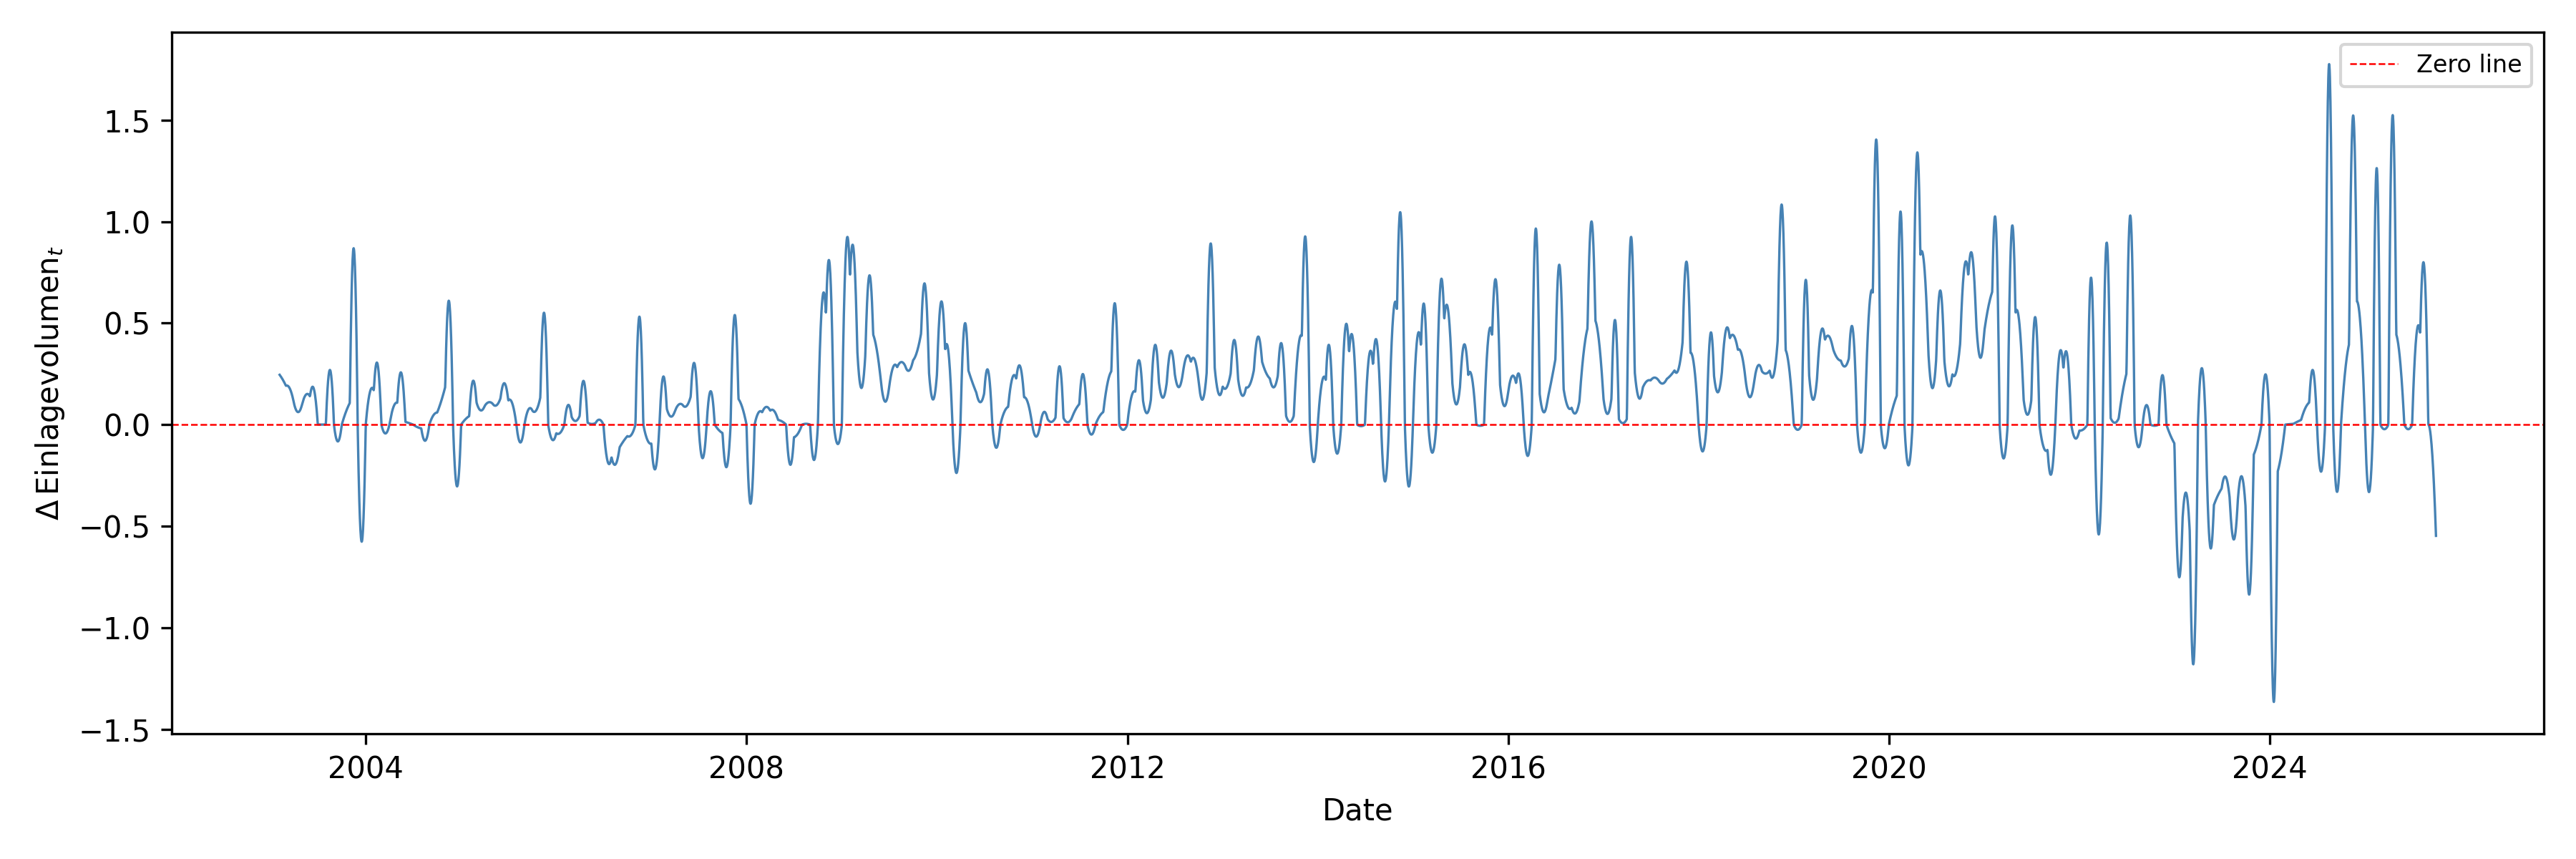
\includegraphics[width=\textwidth]{diff_volume.png}
    \caption{First difference of the deposit volume, $\Delta y_t$, in EUR
    billions per day (vertical axis) over the full sample period January 2003
    -- September 2025 (horizontal axis). The series fluctuates around zero
    throughout, which is consistent with stationarity after differencing.
    Increased volatility from 2022 onward coincides with the ECB interest-rate
    tightening cycle.}
    \label{fig:diff_volume}
\end{figure}

After interpolation to daily frequency, the dataset comprises $8{,}276$ daily
observations covering January 2003 to September 2025. Because the target is
published monthly, these daily rows correspond to approximately $273$
independent monthly releases. The effective sample size is therefore roughly
thirty times smaller than the nominal number of rows, a point we return to in
Section~\ref{subsec:limitations}.

% ---------------------------------------------------------------------------
% 4. Forecasting Models
% ---------------------------------------------------------------------------
\section{Forecasting Models}
\label{sec:models}
\subsection{Forecasting Framework}
\label{sec:framework}

We define \(y_t\) as the volume of German household overnight deposits at time
\(t\), and \(\mathbf{x}_t\) as the vector of our predictors and their lagged values from Equation~\eqref{eq:forecasting_problem}. The objective is to forecast deposit volumes over a
100-day horizon ($H=100$) using the information available during the preceding 100
days ($L=100$). The reasoning for $H=100$ is because it accounts for roughly one quarter of trading days, therefore relevant for the operational liquidity management's planning cycle. 

At time of forecast \(t\) the information set contains the historical deposit volume and the
selected covariates over the period \(t-L+1,\ldots,t\). Each model produces
the complete vector of predicted changes for the following \(H=100\) days:
\begin{equation}
    \widehat{\boldsymbol{\Delta y}}_{t+1:t+H}
    =
    f\!\left(
        y_{t-L+1:t},
        \mathbf{x}_{t-L+1:t}
    \right),
    \qquad L=100,\quad H=100.
    \label{eq:forecasting_problem}
\end{equation}

%Setting $L = H$ follows the common convention that the context available to a
%multi-horizon forecaster should be at least as %long as the horizon it must
%predict \citep{lim2021, zeng2023transformers}. %Also, since the deposit
%series is published monthly and interpolated to a %daily grid
%(Section~\ref{subsec:interpolation}), a window of %100 trading days spans
%approximately five genuine monthly observations %of the target and provides the models with recent %information. 
\begin{comment}
Finally, even a 100-day window does not span an annual cycle of approximately
250 trading days, so no model in this comparison can learn calendar
seasonality or multi-year interest-rate cycles from its encoder input. This
restriction applies identically to all models and therefore does not bias the
comparison between them, but it does bound what any of them could in principle
achieve; Section~\ref{subsec:limitations} treats it as a threat to the
external validity of our conclusion.
\end{comment}

A direct multi-output forecasting strategy is used for this study. Each model
estimates all 100 future changes simultaneously rather than recursively one
day at a time. The predicted changes are then converted back into
deposit-volume levels according to
\begin{equation}
    \widehat{y}_{t+h}
    =
    y_t+
    \sum_{j=1}^{h}
    \widehat{\Delta y}_{t+j},
    \qquad h=1,\ldots,H.
    \label{eq:level_reconstruction}
\end{equation}


\indent Only information available up to time $t$ is used for model estimation
and for fitting the feature scaler, which is a robust scaler estimated on the
training window alone. Actual covariate values within the 100 forecast days
are never used. For the TFT, covariates are held constant at their most
recently observed value over the horizon, while date-based variables that are
known in advance are supplied for the entire forecast horizon.

\subsection{Model Specifications}

\paragraph{Naive benchmarks.}
The one-step drift benchmark extrapolates the latest daily change,
\[
\hat{y}_{t_0+h}=y_{t_0}+h\Delta y_{t_0},
\]
whereas the constant-level benchmark sets
\(\hat{y}_{t_0+h}=y_{t_0}\).
\begin{comment}
%Both benchmarks are fully interpretable, require
%no covariates, and serve as the reference against which the estimated models
%are compared.  Because the interpolated target is locally very smooth
(Section~\ref{subsec:interpolation}), the one-step drift benchmark is a
demanding reference at short horizons and a fragile one at long horizons,
which is visible in the results.\end{comment}

\paragraph{Linear regression (Ridge).}
A multi-output ridge regression maps the flattened 100-day lookback window to
the 100-step forecast vector, regularized by an $\ell_2$ penalty $\alpha$. As a linear model, Ridge yields
directly inspectable coefficients. Also, the flattened feature vector is
high-dimensional and strongly collinear, so it makes shrinkage adequate.

\paragraph{XGBoost.}
Gradient-boosted regression trees are trained on the same flattened input
representation \citep{chen2016}, with maximum depth, learning rate and
subsample ratio selected by chronological time-series cross-validation.
Boosted trees can capture non-linear covariate interactions that Ridge cannot
\citep[Ch.~10]{hastie2009}, while remaining moderately interpretable.

\paragraph{Feedforward neural network (FFN).}
The FFN is a multilayer perceptron with ReLU activations that predicts the
100-step output vector directly. Its layer configuration and $\ell_2$
penalty are selected using the same chronological cross-validation procedure
and tuning budget as Ridge and XGBoost
(Section~\ref{subsec:tuning}). Training uses the Adam optimizer and early
stopping on the final $15\%$ of the training window, with a patience of
20 epochs and a maximum of 500 epochs. The chronological validation split
preserves the time ordering of the observations, although adjacent 100-day
sequences may still overlap.

\paragraph{Temporal Fusion Transformer (TFT).}
The TFT explicitly
distinguishes between known future inputs (calendar features: weekday, month-end indicator,
day-of-month) and unknown future inputs (the six macro-financial covariates). The encoder length is set to $L=100$ to match
the other models, and the model is trained with early stopping on validation
loss with a patience of five validation checks. Despite being the most complex
model considered, its attention mechanism was explicitly designed to offer a
degree of interpretability that purely black-box models lack.

\medskip
Each model is fitted \(S=5\) times to form an ensemble. Ridge, FFN and XGBoost
use bootstrap-resampled training sequences together with different random
seeds; repeated TFT fits differ in the random seed only. Ensemble members are
combined by averaging their forecasts.

\subsection{Tuning Protocol}
\label{subsec:tuning}

A comparison of ``complex'' against ``simple'' models is only meaningful if
the models receive comparable optimisation effort. We therefore impose a
single tuning budget of at most twelve grid configurations per model, searched
by grid search with a three-fold chronological \texttt{TimeSeriesSplit} and
mean absolute error as the selection criterion. Hyperparameters are re-tuned
at every forecast origin using only data available at that origin, so that no
configuration selected on a later window is transferred to an earlier one.
Table~\ref{tab:hyperparams} documents the complete search space.
\begin{comment}; the TFT
architecture is fixed a priori at the configuration shown, since a grid search
over the transformer was not computationally feasible within the same budget.
This asymmetry may disadvantage the TFT relative to the grid-searched models
and is therefore considered a limitation in ~\ref{subsec:limitations}.
\end{comment}

\begin{table}[htbp]
    \centering
    \small
    \caption{Hyperparameter search spaces and fixed settings.}
    \label{tab:hyperparams}
    \begin{tabularx}{\textwidth}{l X c}
        \toprule
        Model & Search space / fixed settings & Configurations \\
        \midrule
        Ridge & $\alpha \in \{10^{-3}, \dots, 10^{3}\}$, 8 values log-spaced & 8 \\
        FFN & hidden layers $\in \{(64,32),(128,64)\}$;
              $\ell_2$ penalty $\in \{10^{-4}, 10^{-3}\}$;
              Adam, learning rate $10^{-3}$;
              early stopping, patience 20 epochs, max.\ 500 & 4 \\
        XGBoost & max.\ depth $\in \{3,4,5\}$;
                  learning rate $\in \{0.05, 0.1\}$;
                  subsample $\in \{0.7, 0.9\}$;
                  50 trees during search, 100 at final fit & 12 \\
        TFT & fixed: hidden size 32, 4 attention heads, dropout $0.1$,
              continuous hidden size 16, Adam, learning rate $10^{-3}$,
              batch size 64, max.\ 40 epochs, early stopping patience 5,
              MAE loss & --- \\
        \midrule
        \multicolumn{3}{l}{\textit{Shared:} $L=100$, $H=100$, $S=5$ ensemble
        members, robust scaling fitted on training window, seed $42$.} \\
        \bottomrule
    \end{tabularx}
\end{table}

\subsection{Covariate Specifications}
\label{subsec:covariates}

To compare how different types of economic information affect forecast
accuracy, each non-naive model is evaluated with the nine covariate sets
listed in Table~\ref{tab:covariate_sets}. These include grouped economic
variables, individual interest-rate variables, and subsets of the full
predictor set. For Ridge, the FFN and XGBoost, each covariate is supplemented
with lags of 1, 5 and 20 calendar days, as defined in
Equation~\eqref{eq:laggedcoveq}. The TFT instead uses the selected covariates
as sequential inputs and does not require these additional lagged features.
The ``Code label'' column gives the identifier used in the code and figure
filenames.

\begin{table}[htbp]
    \centering
    \small
    \caption{Covariate specifications.}
    \label{tab:covariate_sets}
    \begin{tabularx}{\textwidth}{l X l}
        \toprule
        Specification & Included variables & Code label \\
        \midrule
        All & \estr, deposit rate, geopolitical risk, inflation, DAX,
        and ten-year German government bond yield & \texttt{alle} \\
        Interest rates & \estr{} and deposit rate & \texttt{nur\_zinsen} \\
        Financial markets & DAX and ten-year government bond yield &
        \texttt{nur\_maerkte} \\
        Macroeconomic & Geopolitical risk and inflation & \texttt{nur\_makro} \\
        Rates and macroeconomy & \estr, deposit rate, geopolitical risk,
        and inflation & \texttt{zinsen\_makro} \\
        Excluding DAX & All variables except DAX & \texttt{ohne\_dax} \\
        Excluding inflation & All variables except inflation &
        \texttt{ohne\_inflation} \\
        \estr{} only & \estr & \texttt{nur\_estr} \\
        Deposit rate only & Deposit rate & \texttt{nur\_einlagezins} \\
        \bottomrule
    \end{tabularx}
\end{table}

\subsection{Rolling-Origin Evaluation}
\label{subsec:rolling_evaluation}

Forecasting performance is evaluated using an expanding-window rolling-origin
design. At each origin \(o_k\), all observations available up to that date form
the training sample, and the following \(H=100\) days form the evaluation
window:
\begin{equation*}
    \mathcal{T}_k=\{1,\ldots,o_k\},
    \qquad
    \mathcal{E}_k=\{o_k+1,\ldots,o_k+H\}.
\end{equation*}
Models and hyperparameters are re-estimated at every origin. The four origins
are 1 January 2009, 1 January 2013, 1 March 2019, and 1 June 2025, representing
the financial crisis, the low-interest-rate period, the pre-COVID period, and
the post-2022 tightening cycle. The 2009 origin has the shortest training
history.
\begin{comment}The price of this design choice is a very small
number of evaluation points, which we address directly in
Sections~\ref{subsec:evaluation_metrics} and~\ref{subsec:selection}.
\end{comment}

\subsection{Evaluation Metrics}
\label{subsec:evaluation_metrics}

Performance is evaluated for both the predicted first differences and the
reconstructed deposit-volume levels. Let \(y_{k,h}\) and \(\widehat{y}_{k,h}\)
denote the observed and predicted volume at horizon \(h\) after origin
\(o_k\). The metrics are
\begin{align*}
    \operatorname{MAE}_k
    &=
    \frac{1}{H}
    \sum_{h=1}^{H}
    \left|y_{k,h}-\widehat{y}_{k,h}\right|, \\
    \operatorname{RMSE}_k
    &=
    \sqrt{
        \frac{1}{H}
        \sum_{h=1}^{H}
        \left(y_{k,h}-\widehat{y}_{k,h}\right)^2
    }, \\
    R_k^2
    &=
    1-
    \frac{
        \sum_{h=1}^{H}
        \left(y_{k,h}-\widehat{y}_{k,h}\right)^2
    }{
        \sum_{h=1}^{H}
        \left(y_{k,h}-\overline{y}_k\right)^2
    },
\end{align*}
where \(\overline{y}_k\) is the mean observed volume in evaluation window
\(k\). Negative \(R^2\) values indicate performance below the test-window mean
benchmark.

\paragraph{A scale-free measure.}
Absolute MAE is not directly comparable across forecast origins because the
deposit stock increases over time. We therefore scale each model's MAE by the
constant-level benchmark at the same origin:
\begin{equation}
    \operatorname{relMAE}_k
    =
    \frac{\operatorname{MAE}_k^{\text{model}}}
         {\operatorname{MAE}_k^{\text{constant-level}}}.
    \label{eq:relmae}
\end{equation}
Values below one indicate improvement over the benchmark
\citep{hyndman2006mase}. Metrics are reported as mean and standard deviation
across the four origins, with origin-level results in
Appendix~\ref{app:additional}. Because four origins provide little power for
formal forecast-comparison tests, all comparisons are descriptive.

\begin{comment}
\paragraph{Reporting.}
Metrics are calculated separately at each forecast origin and summarised by
their mean and standard deviation across origins. Because only four origins
are available, the complete origin-level results are also reported in
Appendix~\ref{app:additional}. The primary comparison uses MAE on the reconstructed levels and
$\operatorname{relMAE}$; RMSE and \(R^2\) provide complementary information,
and metrics on first differences serve as diagnostics. A Diebold--Mariano test
\citep{dieboldmariano1995} with the small-sample correction of
\citet{harvey1997} was implemented but is deliberately not applied to the main
results: with four origins the test has essentially no power.
Model comparisons are therefore reported descriptively throughout.
\end{comment}

% ---------------------------------------------------------------------------
% 5. Results
% ---------------------------------------------------------------------------
\section{Results}
\label{sec:results}

\subsection{Forecasting Performance}

Table ~\ref{tab:overall_results} reports the forecasting performance of each model. The covariate
specification with the lowest mean level MAE across the four origins, together
with the scale-free measure of Equation~\eqref{eq:relmae} is specified.

\begin{table}[htbp]
\centering
\small
\caption{Forecasting performance across the four rolling origins (2009, 2013,
2019, 2025). With MAE and RMSE measured in EUR billions and reported as mean
$\pm$ standard deviation across origins.}
\label{tab:overall_results}
\begin{tabularx}{\textwidth}{l X c c c c}
\toprule
Model & Best covariate set & MAE & RMSE & Mean $R^2$ & relMAE \\
\midrule
\multicolumn{6}{l}{\textit{Estimated models}}\\[2pt]
Ridge
& All covariates
& $9.36 \pm 11.11$
& $10.26 \pm 12.08$
& $0.178$
& $0.44 \pm 0.31$ \\

TFT
& Macroeconomic
& $10.78 \pm 12.61$
& $12.71 \pm 14.18$
& $-0.361$
& $0.49 \pm 0.39$ \\

FFN
& Macroeconomic
& $11.85 \pm 6.90$
& $15.22 \pm 10.35$
& $-0.605$
& $0.71 \pm 0.34$ \\

XGBoost
& Excluding inflation
& $12.71 \pm 13.28$
& $14.90 \pm 14.79$
& $-0.784$
& $0.69 \pm 0.64$ \\
\midrule
\multicolumn{6}{l}{\textit{Naive benchmarks}}\\[2pt]
One-step drift
& None
& $11.78 \pm 12.81$
& $14.41 \pm 14.25$
& $-0.564$
& $0.60 \pm 0.43$ \\

Constant level
& None
& $17.38 \pm 10.13$
& $21.03 \pm 10.52$
& $-2.246$
& $1.00$ \\
\bottomrule
\end{tabularx}
\vspace{2pt}
\parbox{\textwidth}{\footnotesize
\textit{Note:} MAE and RMSE are calculated on reconstructed deposit-volume
levels. relMAE is the MAE relative to the constant-level benchmark at the same
origin; values below one indicate improvement over that benchmark.
}
\end{table}

Ridge achieved the lowest average MAE and was the only approach with a
positive mean $R^2$. The TFT ranked second, followed by the one-step drift
benchmark. Neither the FFN nor XGBoost improved on that simple benchmark on
average, and the constant-level forecast produced the largest errors. Greater model complexity therefore did not consistently translate into higher
forecasting accuracy. 

\paragraph{Answering RQ1.}
Forecast accuracy is determined mainly by the $\operatorname{relMAE}$, since
absolute errors are affected by the level of the deposit stock. Over the
100-day horizon, Ridge records an error equal to $44\%$ of the constant-level
benchmark. The one-step drift benchmark records $60\%$, while XGBoost and the
FFN record $69\%$ and $71\%$, respectively. Thus, all methods improve on the
constant-level benchmark, although Ridge's improvement over the one-step
drift forecast is smaller. Figure~\ref{fig:model_comparison} also shows that the
standard-deviation bars overlap almost completely, which is the visual form of
the statistical caveat stated in Section~\ref{subsec:evaluation_metrics}: with
four origins, this ranking describes a sample, not a population.

\begin{figure}[htbp]
    \centering
    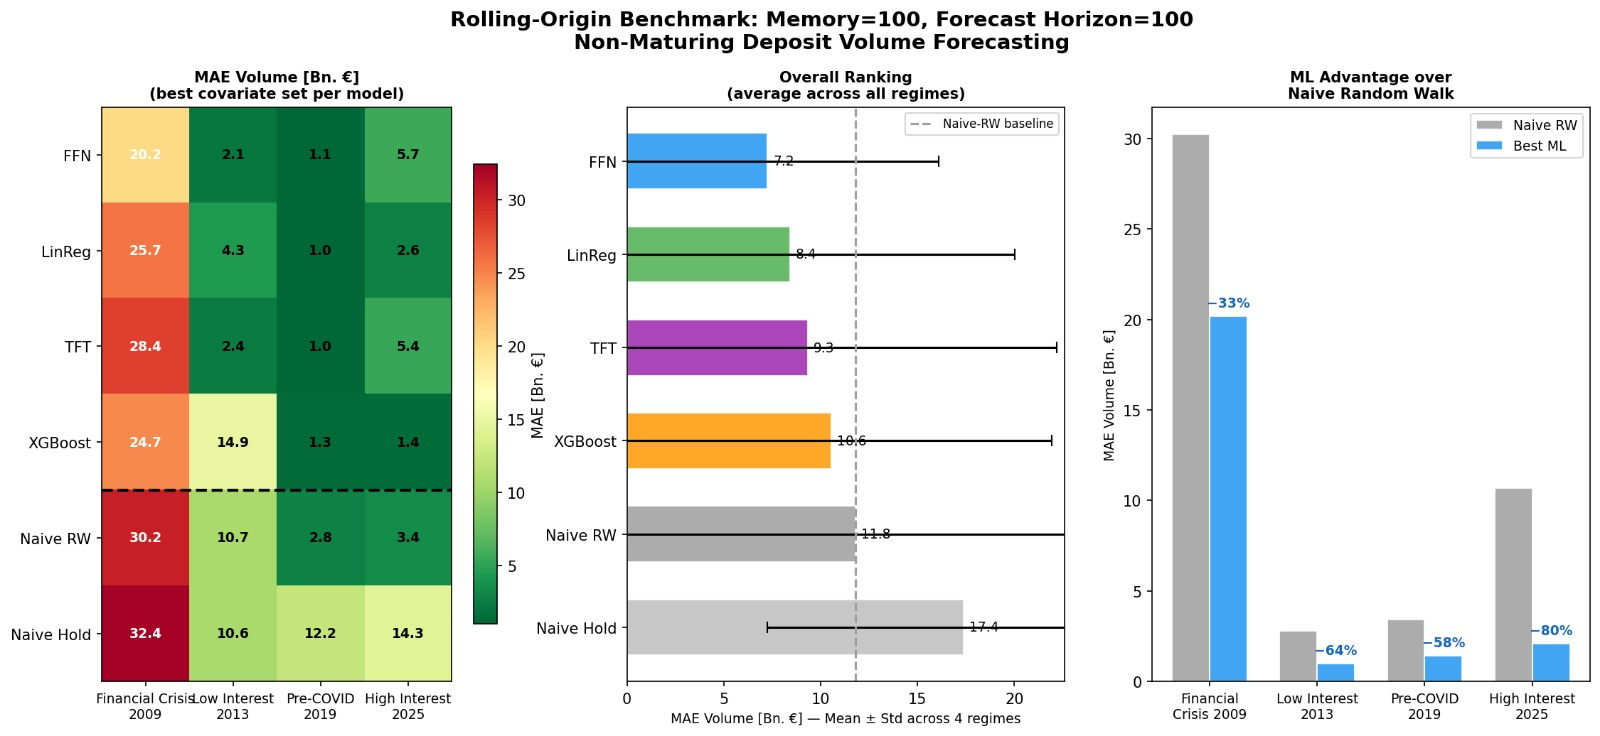
\includegraphics[width=0.95\textwidth]{model_comparison.jpeg}
    \caption{Mean MAE of reconstructed deposit-volume levels across the four
forecast origins (2009, 2013, 2019 and 2025). Each model is shown using its
lowest-MAE covariate specification, and error bars indicate one standard
deviation across origins. The horizontal line marks the one-step drift
benchmark.}
    \label{fig:model_comparison}
\end{figure}



\subsection{Accuracy Versus Robustness}

\begin{figure}[htbp]
    \centering
    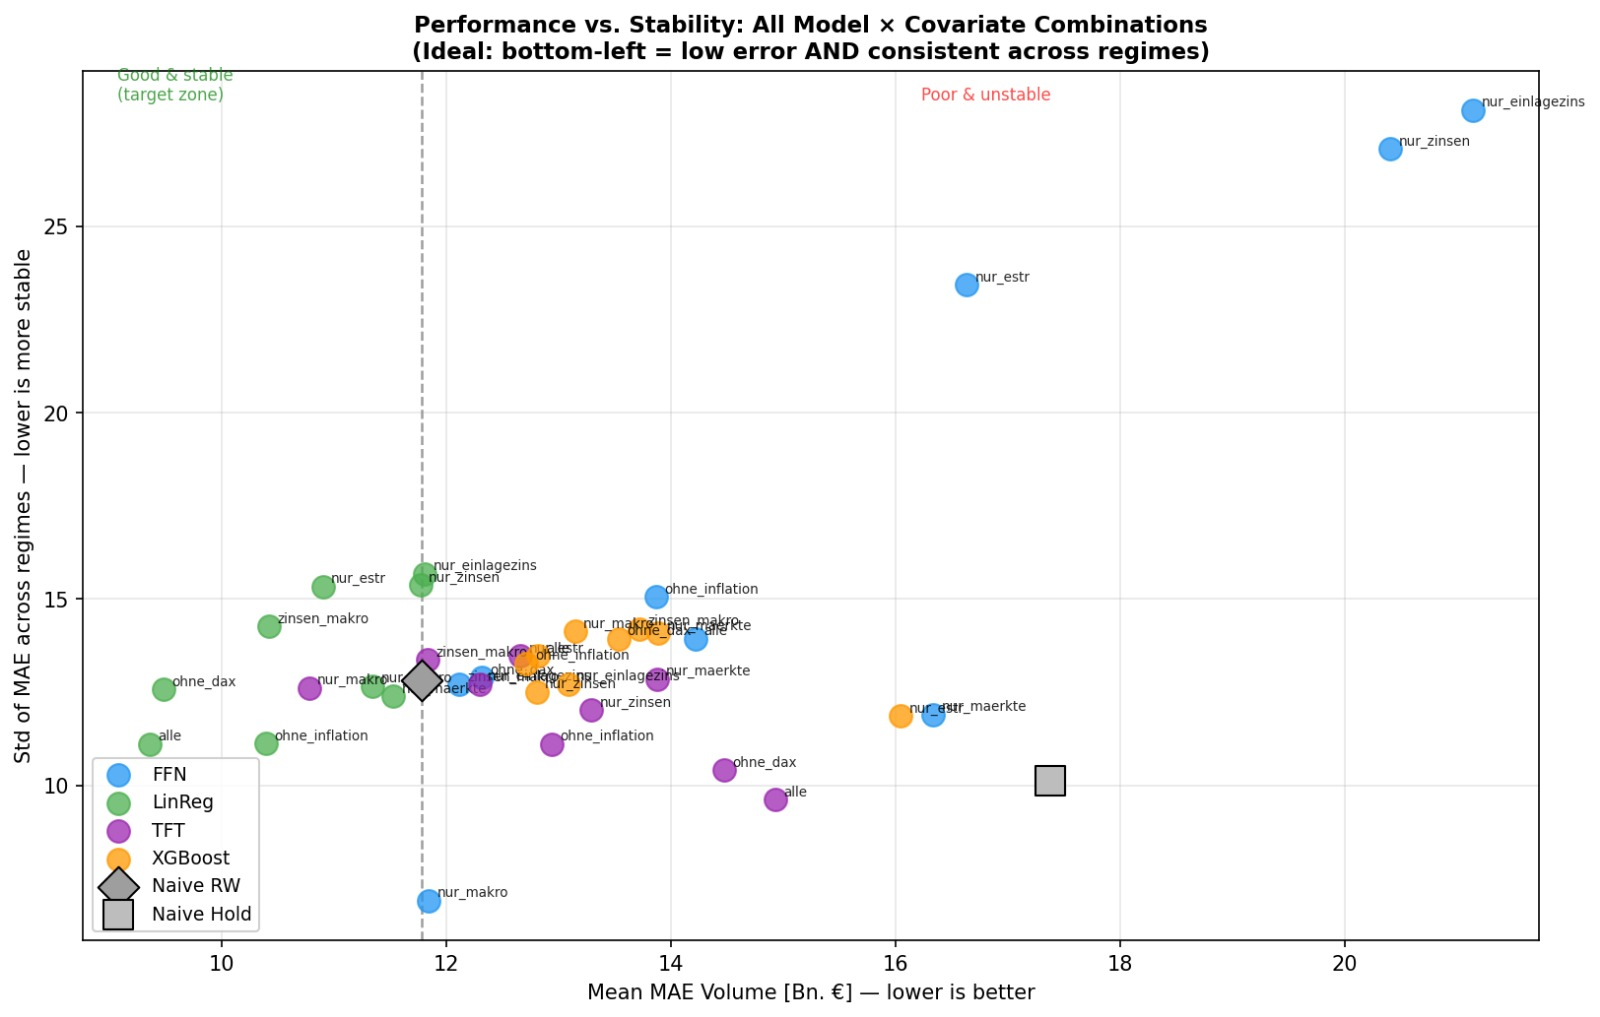
\includegraphics[width=0.85\textwidth]{performance_vs_stability.jpeg}
    \caption{Forecast accuracy and stability across all model--covariate
combinations. The horizontal axis shows mean level MAE across the four
forecast origins, while the vertical axis shows its standard deviation.
Lower values indicate greater accuracy and stability. The dashed lines mark
the mean MAE and standard deviation of the one-step drift benchmark.}
    \label{fig:perf_vs_stability}
\end{figure}

Figure~\ref{fig:perf_vs_stability} compares forecast accuracy and stability
for all model-covariate combinations. Ridge has the most specifications lying on the lower-left region, indicating both lower mean MAE and lower dispersion
than the one-step drift benchmark. Ridge is the most accurate model across covariate specifications, whereas the FFN specification using
macroeconomic covariates has the lowest absolute dispersion
($\pm 6.90$).

However, after normalising errors by the constant-level benchmark, Ridge
achieves the lowest dispersion among the selected models
($0.31$ in $\operatorname{relMAE}$), followed by the FFN ($0.34$) and 
XGBoost ($0.64$). Moreover, XGBoost achieves an average
$\operatorname{relMAE}$ of $0.69$, compared with $0.71$ for the FFN. This
shows why absolute errors are not directly comparable across forecast origins
with different deposit levels.

\subsection{Effect of Covariate Selection}

The preferred covariate specification differs across models, as reported in
Table~\ref{tab:overall_results}. The complete results for all nine
specifications are presented in
Figure~\ref{fig:covariate_results_full} in the appendix.

Ridge is comparatively stable, with mean MAE ranging from $9.36$ to
$11.81$ EUR bn across the nine specifications. This corresponds to an
increase of $26.2\%$ from its best to its worst specification. XGBoost shows
a similar increase of $26.3\%$, with mean MAE ranging from $12.71$ to
$16.05$ EUR bn. The TFT is more sensitive, ranging from $10.78$ to
$14.93$ EUR bn, an increase of $38.5\%$. The FFN is the most sensitive to
the selected covariates, with mean MAE ranging from $11.85$ to
$21.14$ EUR bn, an increase of $78.4\%$.

Ridge's relatively narrow range is consistent with the effect of
$\ell_2$ regularization, which shrinks the coefficients of weakly informative
predictors towards zero. For Ridge, the FFN and XGBoost, changing the
covariate specification also changes the size of the flattened input vector.
With a 100-day lookback and the current value together with lags of 1, 5 and
20 days, each additional covariate contributes 400 input values. This increase
in dimensionality may partly explain the greater sensitivity of the FFN. The
TFT processes the covariates sequentially and is therefore not affected by
the flattened input dimension in the same way.

Overall, the results show that adding more predictors does not necessarily
improve forecast accuracy. The selected specifications describe predictive
performance within this sample and should not be interpreted as evidence of
causal relationships between the covariates and deposit volumes..

\subsection{Variation Across Forecast Origins}

Forecast accuracy varies considerably across the four evaluation periods.
Over the six methods reported in Table~\ref{tab:overall_results},
the average mean level MAE is approximately $27.9$ Bn.\ EUR at the 2009 origin, compared
with $3.6$, $8.3$, and $9.4$ Bn.\ EUR at the 2013, 2019, and 2025 origins,
respectively. The 2009 period accounts for a substantial part of the
dispersion in the aggregate results. This origin combines the global financial
crisis with the smallest available training sample. Given the $L=100$
lookback and $H=100$ forecast horizon, the effects of the economic regime and
limited training history cannot be separated completely.

\begin{figure}[htbp]
    \centering
    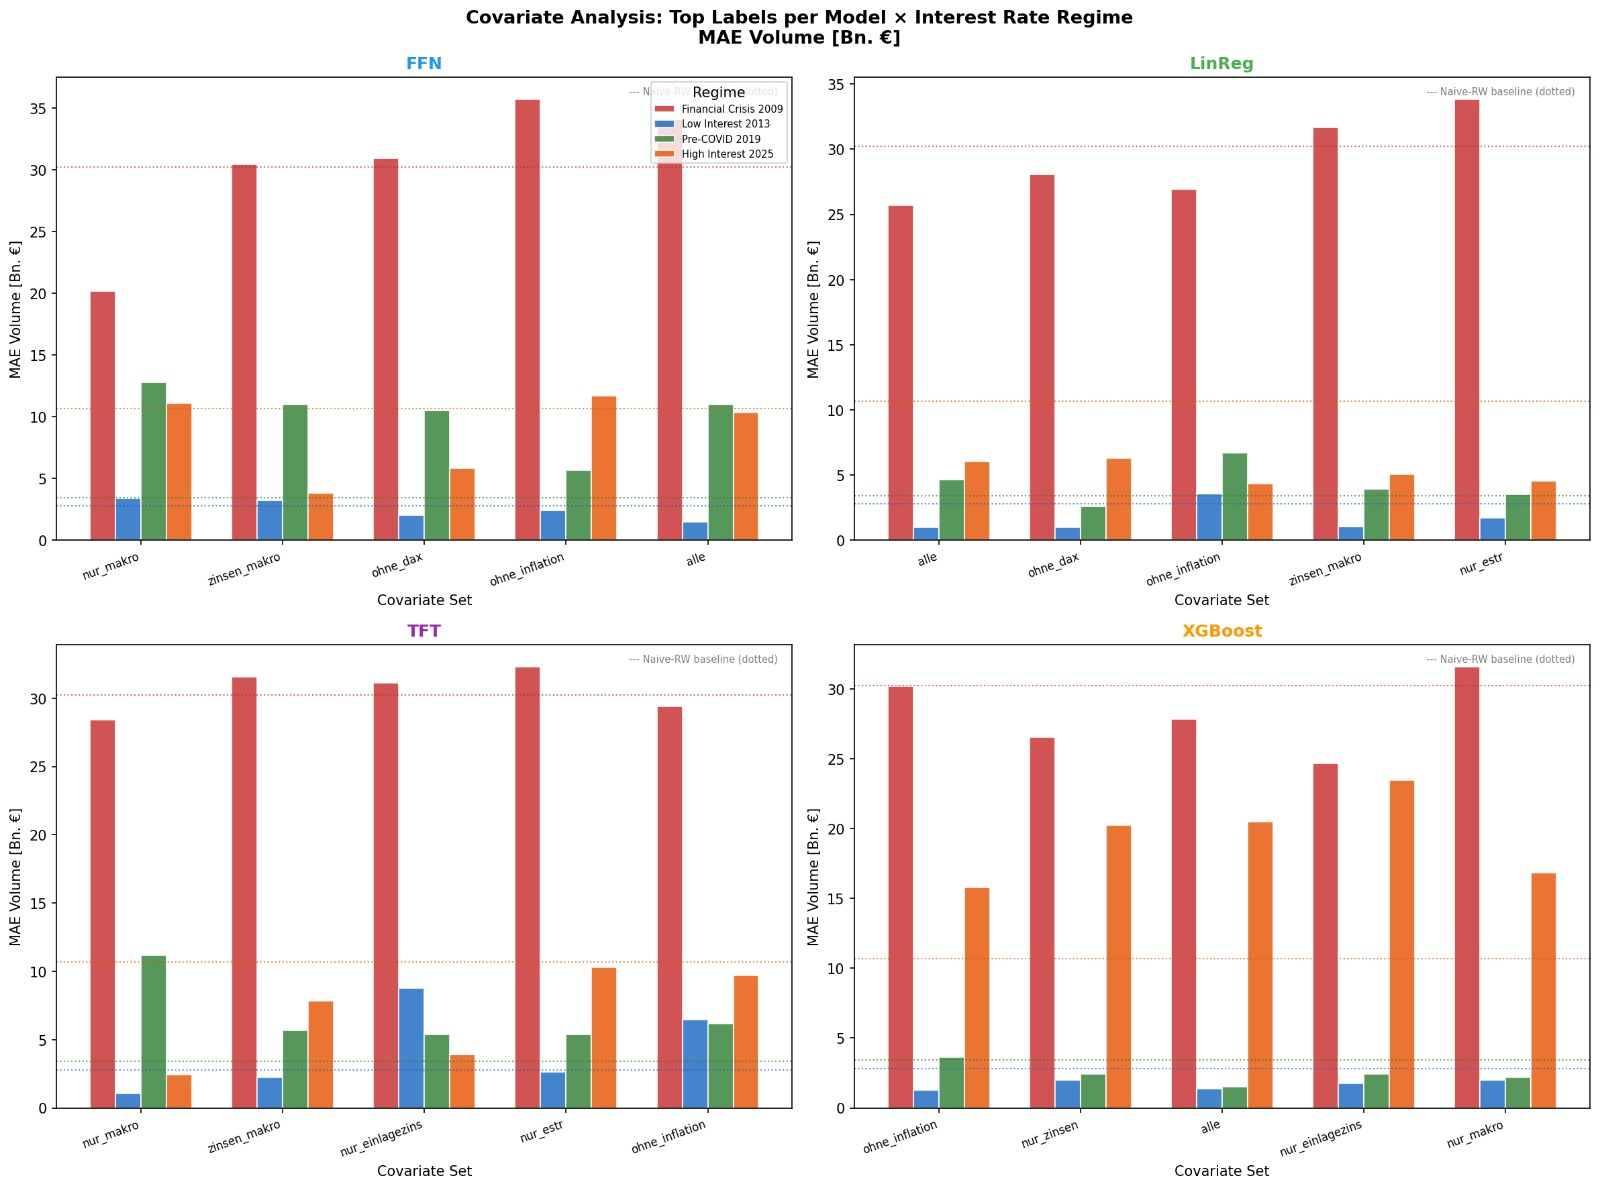
\includegraphics[width=\textwidth]{mae_per_covariate_per_time.jpeg}
    \caption{Level MAE across covariate specifications, separated by model and
    forecast origin. Each panel represents one model, while the colours identify
    the four forecast origins. Lower values indicate better forecast performance.}
    \label{fig:mae_covariate_time}
\end{figure}

\begin{figure}[htbp]
    \centering
    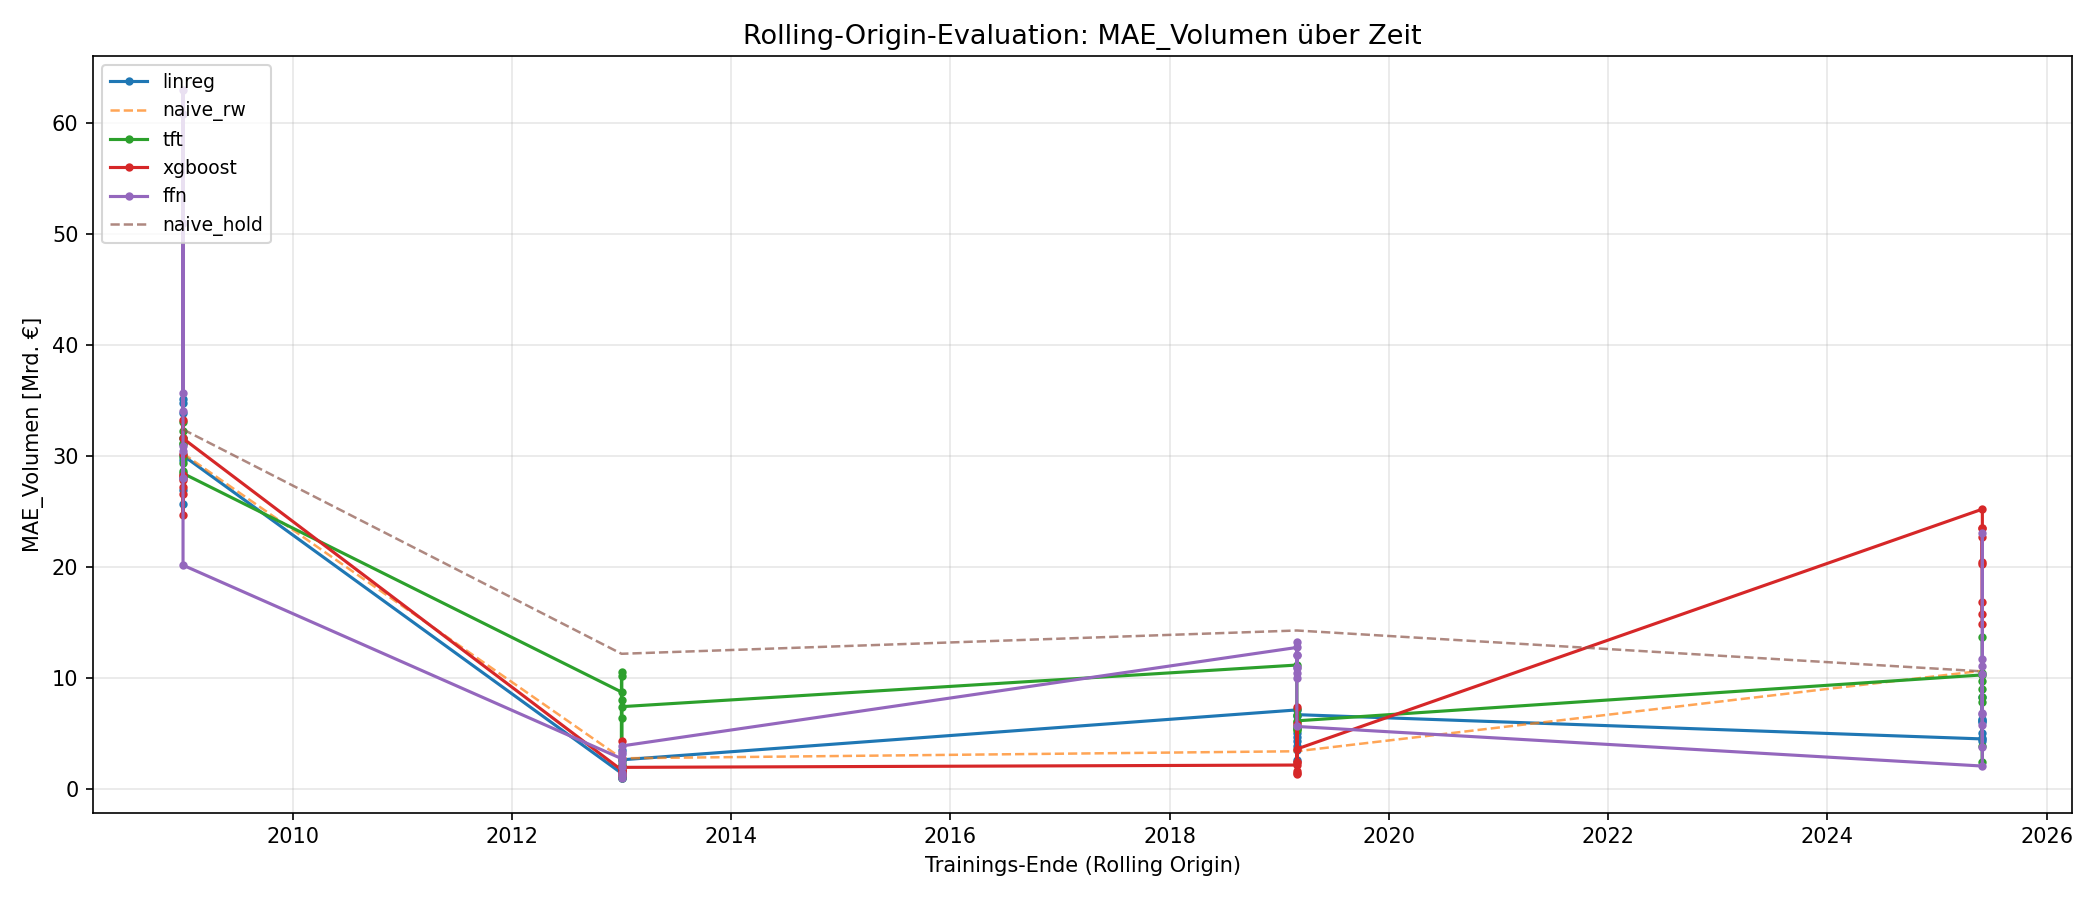
\includegraphics[width=\textwidth]{covariate_benchmark_rolling_timeline.png}
    \caption{Rolling-origin evaluation: level MAE (EUR billions, vertical
    axis) per model plotted against the end of the training window
    (horizontal axis). Naive benchmarks are drawn as dashed reference lines,
    estimated models as solid lines with markers.}
    \label{fig:rolling_timeline}
\end{figure}

\begin{figure}[htbp]
    \centering
    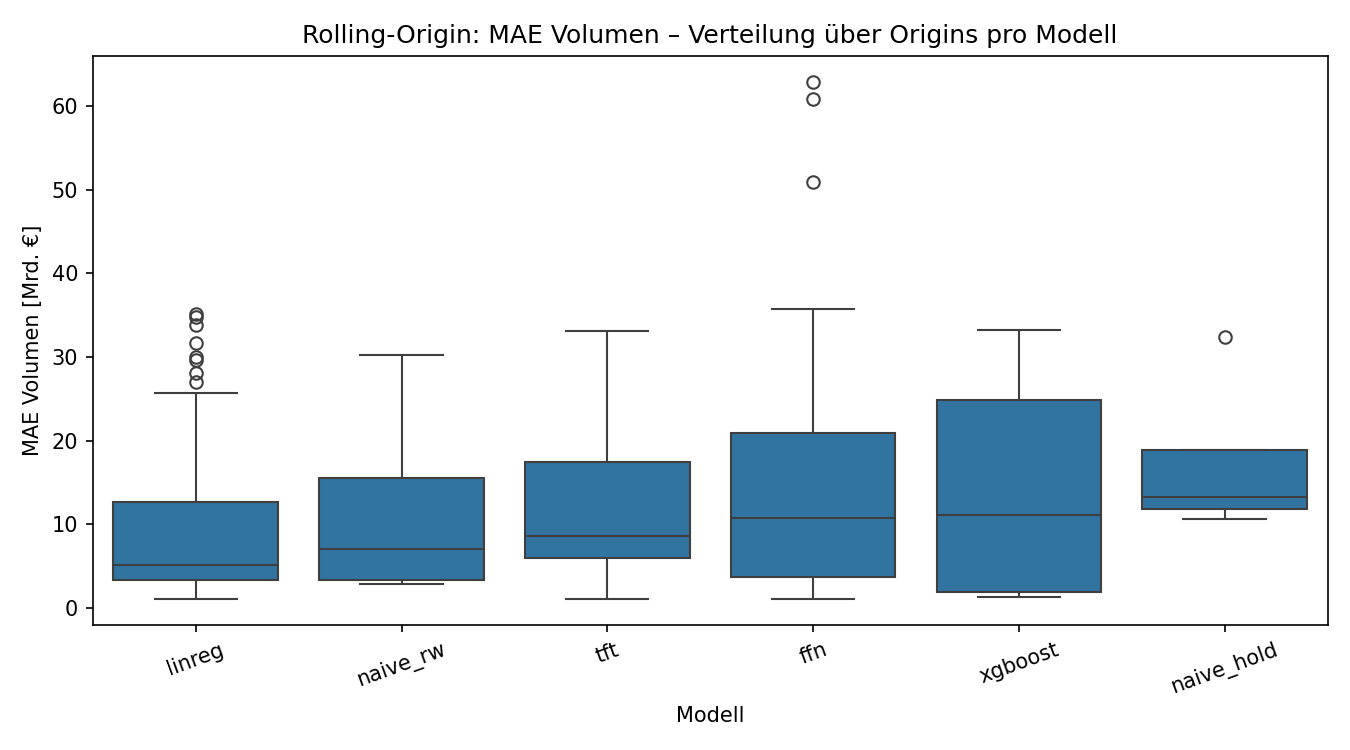
\includegraphics[width=0.85\textwidth]{covariate_benchmark_rolling_summary.png}
    \caption{Distribution of level MAE (EUR billions, vertical axis) across
    the four rolling origins per model, shown as boxplots ordered by median.
    Box height reflects the interquartile range, whiskers the full observed
    range across origins.}
    \label{fig:rolling_summary}
\end{figure}

Both figures~\ref{fig:mae_covariate_time} and \ref{fig:rolling_timeline} show
that no model dominates across all forecast origins. The FFN records the
lowest error in 2009, Ridge performs best in 2013 and remains competitive in
2019 and 2025, while the TFT records the lowest error at the 2025 origin.
Moreover, the best-performing covariate specification changes across origins
for every model. The aggregate rankings should then be interpreted as average performance across different economic periods, rather than as evidence that one model or covariate specification is consistently superior.

\subsection{Interpreting the Selection Procedure}
\label{subsec:selection}

Each estimated model is reported using the best
of nine covariate sets selected on the same four origins used for evaluation,
which may overstate its advantage over the untuned naive benchmarks. The
origins were chosen deliberately rather than sampled randomly, and standard
deviations based on four observations are imprecise. The results therefore do
not establish universal Ridge superiority, but they provide no evidence that
greater complexity consistently improves forecast accuracy.







%%%%%%%%%%%%%%%%%%%%%%%%%%%%%%%%%%%%%%%%%%%%%%%%%%%%%%%%%%%%%%%%%%%%%%%%%%%%%
% ---------------------------------------------------------------------------
% 6. Discussion
% ---------------------------------------------------------------------------
\section{Discussion}
\label{sec:discussion}

The rolling-origin benchmark shows that an $\ell_2$-regularized linear model (Ridge) achieved lower overall prediction error across the 100-day horizon than the more complex non-linear architectures. This section analyzes the causes of these performance differences, links the forecasts to the underlying economic regimes, and details the limitations of our framework.

\subsection{Ridge Regression}
Ridge achieved the highest overall accuracy ($\text{MAE} = 9.36\text{ Bn EUR}$, $\operatorname{relMAE} = 0.44$), outperforming the drift baseline by roughly 20\%. It was also the only model with a positive mean $R^2$ ($0.178$).

The main advantage of Ridge lies in its shrinkage penalty. Because we calculated level forecasts by adding up predicted daily differences, any small daily bias compounds over a 100-day horizon (for instance, a daily error of just $0.05\text{ Bn EUR}$ turns into a $5\text{ Bn EUR}$ drift by day 100). Over longer horizons, keeping the daily prediction unbiased matters much more than daily variance. The Ridge penalty shrinks noisy parameters toward zero, which stops this cumulative drift.

This heavy regularization was necessary because of the high feature-to-observation ratio. A 100-day lookback window across six covariates and their respective lags creates roughly 2,500 features, while the earliest origin provides only about 1,350 training observations. On top of that, adjacent lags and macro-financial variables (like deposit rates and ten-year yields) are highly correlated. Ridge handles this collinearity by shrinking dependent parameter weights, keeping forecasts stable even when testing different covariate sets.

As shown in Figure~\ref{fig:forecast_linreg}, Ridge residuals remain centered around zero for the 2013, 2019, and 2025 origins. The 2009 financial crisis was the only period where the model developed a systematic forecast bias, caused by the sudden structural shift following the Lehman Brothers collapse.

\originsgrid
  {forecast_linreg_alle_2009-01-01.png}
  {forecast_linreg_alle_2013-01-01.png}
  {forecast_linreg_alle_2019-03-01.png}
  {forecast_linreg_alle_2025-06-01.png}
  {Ridge forecasts with the full covariate set across the four origins.}
  {fig:forecast_linreg}

\subsection{Temporal Fusion Transformer (TFT)}
The TFT ranked second overall ($\text{MAE} = 10.78\text{ Bn EUR}$) and achieved the lowest error of any model at the 2025 origin ($2.43\text{ Bn EUR}$). However, its core strength, using self-attention mechanisms to weigh future inputs, yielded limited benefits in this setup.

To prevent data leakage, future macro variables were held constant across the 100-day evaluation window, with only calendar features updating over time. Because these economic inputs remained static, they provided no dynamic future signals for the TFT decoder. Consequently, the model defaulted to extrapolating previous trends into a smooth path (Figure~\ref{fig:forecast_tft}). This highlights that complex architectures like TFT offer little advantage when exogenous variables cannot be forecasted accurately in advance.

\originsgrid
  {forecast_tft_nur_makro_2009-01-01.png}
  {forecast_tft_nur_makro_2013-01-01.png}
  {forecast_tft_nur_makro_2019-03-01.png}
  {forecast_tft_nur_makro_2025-06-01.png}
  {TFT forecasts using macroeconomic covariates.}
  {fig:forecast_tft}

\subsection{FFN and XGBoost}
Neither FFN ($11.85\text{ Bn EUR}$) nor XGBoost ($12.71\text{ Bn EUR}$) managed to beat the simple drift benchmark ($11.78\text{ Bn EUR}$). They struggled for different reasons:

\begin{itemize}
    \item \textbf{FFN:} It gave consistent but overly smoothed results. It performed surprisingly well during the unpredictable 2009 crisis ($20.18\text{ Bn EUR}$), but failed to get close to the target in easier periods like 2013. Without strong regularization, its dense layer fits noise across individual lag positions.
    \item \textbf{XGBoost:} Decision trees cannot extrapolate trends beyond the ranges seen in training data. This was obvious at the 2025 origin (post-2022 rate hikes), where deposit shifts exceeded historical values. XGBoost flattened out quickly, leading to large accumulation errors ($15.77\text{ Bn EUR}$ vs Ridge's $6.05\text{ Bn EUR}$).
\end{itemize}

\begin{figure}[htbp]
    \centering
    \begin{subfigure}[b]{0.49\textwidth}
        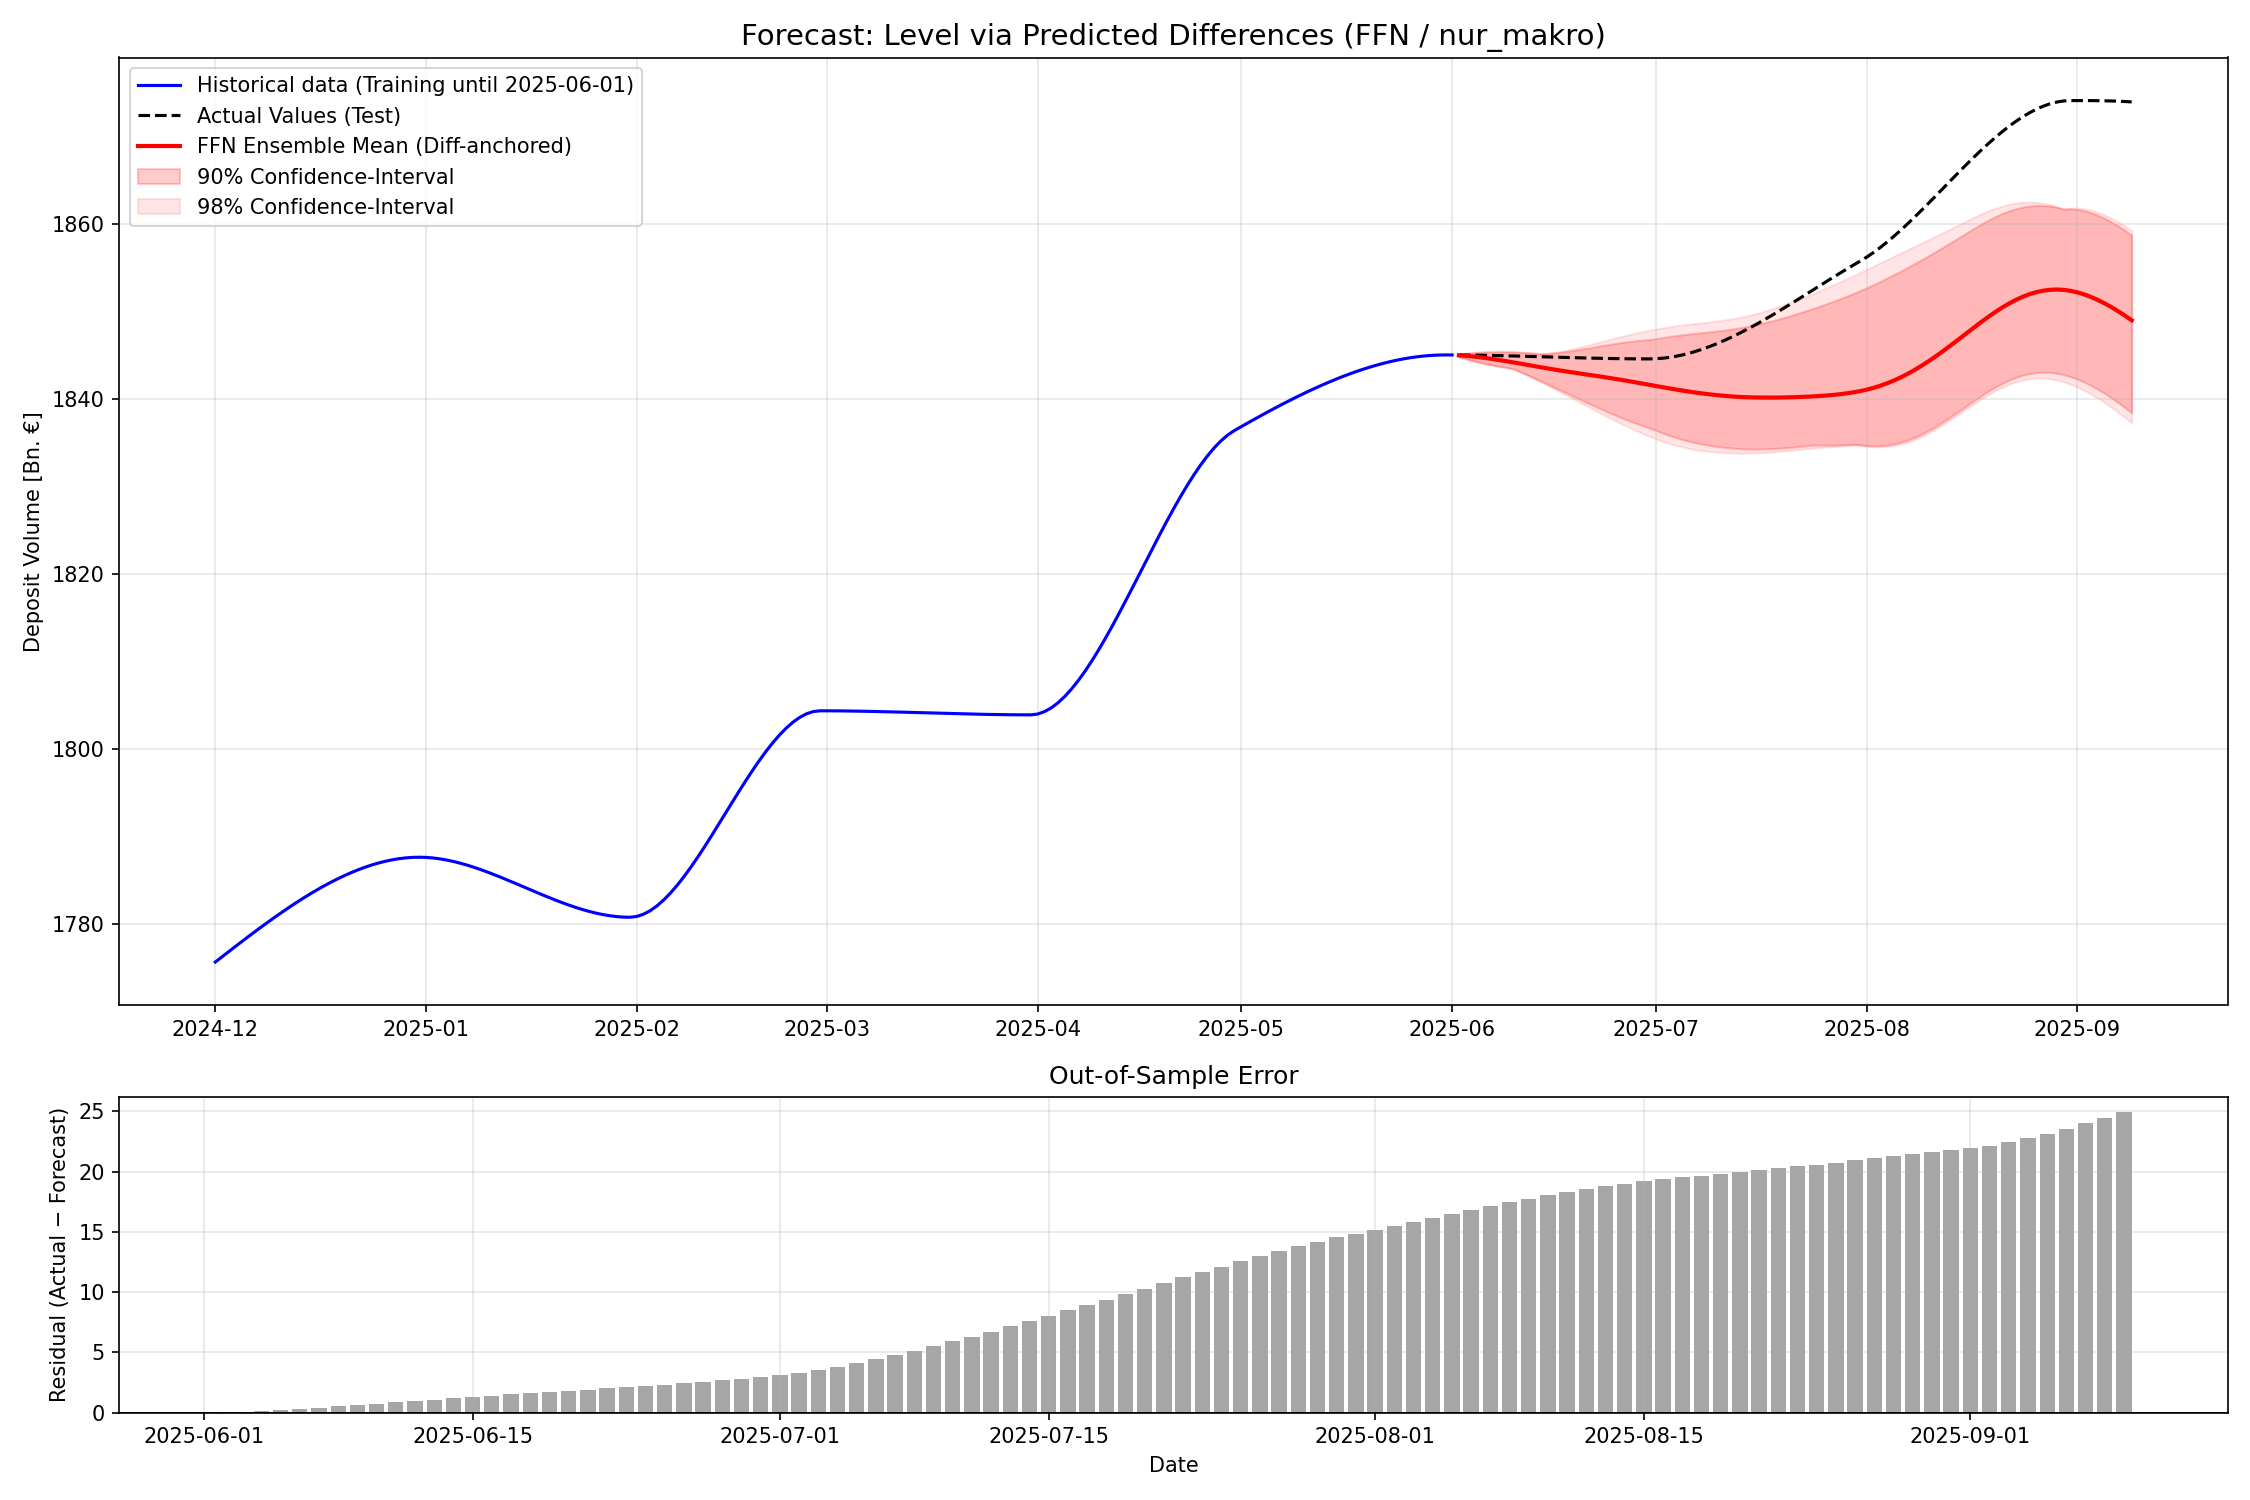
\includegraphics[width=\textwidth]{forecast_ffn_nur_makro_2025-06-01.png}
        \caption{FFN (macro covariates)}
    \end{subfigure}\hfill
    \begin{subfigure}[b]{0.49\textwidth}
        
\includegraphics[width=\textwidth]{forecast_xgboost_nur_einlagezins_2025-06-01.png}
        \caption{XGBoost (deposit rate only)}
    \end{subfigure}
    \caption{Comparing FFN and XGBoost at the June 2025 origin.}
    \label{fig:forecast_nonlinear}
\end{figure}

\subsection{Why 2009 and 2025 Were Difficult to Predict}
\label{subsec:economic}
The largest forecast errors across all models occurred during major structural shifts:
\begin{enumerate}
    \item \textbf{January 2009:} Right after Lehman Brothers collapsed, household behavior was driven by panic, safety guarantees, and flight-to-quality—factors not captured by historical rate series or inflation lags.
    \item \textbf{June 2025:} Post-pandemic savings and rapid ECB rate hikes caused a massive shift from overnight to term deposits. Our models included raw deposit rates, but not the actual rate spread or deposit-beta pass-through speed. Adding an explicit deposit-spread variable would likely fix this.
\end{enumerate}

\subsection{Note on $R^2$ and Study Limitations}
Seeing negative $R^2$ values might look like a red flag at first, but it is actually quite common in multi-step time series forecasting. In these setups, standard $R^2$ compares predictions to a flat average of the future test period—a line no real-time model could actually know. Since all our models beat the constant baseline ($\operatorname{relMAE} < 1.0$), they clearly hold predictive value despite the negative $R^2$.

A few practical limitations of our study should be noted:
\begin{itemize}
    \item \textbf{Interpolated Target Data:} The target deposit volume is published monthly and interpolated to daily frequency. This makes daily steps smooth, which slightly favors simpler extrapolative methods.
    \item \textbf{Limited Evaluation Origins:} Testing on only four dates limits formal statistical testing.
    \item \textbf{Sector-level Data:} We use aggregate Bundesbank data. While good for macro insights, individual banks have unique customer spreads and deposit dynamics that aggregate data masks.
\end{itemize}

\subsection{Key Takeaways}
For bank asset-liability management (ALM) and practical forecasting applications, our results suggest three main conclusions:
\begin{enumerate}
    \item \textbf{Linear models are hard to beat in practice:} Regularized models like Ridge are fast to compute, easy to explain, and give high stability over 100-day horizons.
    \item \textbf{Complexity doesn't guarantee accuracy:} Moving from no model to a basic statistical model gives a massive jump in accuracy, but upgrading to complex deep learning increases computation time and does not improve accuracy unless rich future features are guaranteed.
    \item \textbf{Model selection depends on the goal:} While Ridge is best for baseline operational forecasting, FFN proved more stable during the 2009 market shock. Using a simple ensemble approach could provide the best balance between daily precision and crisis resilience.
\end{enumerate}
















% ---------------------------------------------------------------------------
% 7. Conclusion and Outlook
% ---------------------------------------------------------------------------
\section{Conclusion and Outlook}
\label{sec:conclusion}

Accurate forecasting of non-maturity deposit (NMD) volumes is fundamental to bank liquidity management, regulatory balance-sheet planning, and interest-rate risk assessment. Modeling aggregate NMDs is challenging: the underlying series is non-stationary, strongly autocorrelated, and vulnerable to macroeconomic shifts. Furthermore, existing literature largely treats deposit volumes as valuation inputs rather than standalone targets evaluated out of sample.

To address this gap, we evaluated six forecasting approaches across four origins spanning distinct interest-rate regimes between 2009 and 2025. Using an expanding-window design with a standard 100-day lookback window and equal tuning budgets, our results answer the three core research questions:

\begin{enumerate}
    \item Across a 100-day horizon, the top-performing model cut the mean absolute error to $44\%$ of the constant-level baseline ($\text{MAE} = 9.36\text{ Bn EUR}$) across all four economic regimes. Notably, performance varied far more across time periods than across model families. The 2009 financial crisis was roughly three times harder to forecast than any other origin, driving most of the overall error dispersion.
    
    \item Added model complexity did not yield better accuracy. Ridge regression achieved the highest overall performance ($\operatorname{relMAE} = 0.44$, mean $R^2 = 0.178$), slightly ahead of the TFT ($0.49$). Meanwhile, XGBoost ($0.69$) and the FFN ($0.71$) failed to beat a simple one-step drift rule ($0.60$). Given our sample size of four evaluation origins, these findings reflect a lack of practical advantage for deep learning rather than definitive superiority of linear models.
    
    \item The usefulness of a covariate set depended more on the model architecture using it than on the data itself. Ridge performance varied by only $26\%$ across specifications and worked best with the full feature set, proving that L2 regularization handles collinear lag matrices effectively. In contrast, FFN error nearly doubled on larger feature sets, performing best on the smallest input subset.
\end{enumerate}

\subsection{Outlook and Future Work}
Based on these findings, we thought of four practical extensions for future research:

\begin{enumerate}
    \item Testing models on actual monthly data, rather than daily interpolated figures, would show how they perform against real, unadjusted observations.
    \item Varying the lookback window ($L \in \{100, 250, 500\}$ days) would reveal if a full year of history helps deep architectures capture seasonal patterns better than a linear model.
    \item Instead of keeping future macro variables flat, using scenario-based projections would give models like TFT actual dynamic signals to work with.
    \item Adding explicit deposit spreads and pass-through speeds (deposit-beta) should yield greater accuracy gains than tweaking model architectures, especially during policy rate shifts.
\end{enumerate}

% ---------------------------------------------------------------------------
% Bibliography
% ---------------------------------------------------------------------------
\bibliographystyle{apalike}
\bibliography{references}

% ---------------------------------------------------------------------------
% Appendices
% ---------------------------------------------------------------------------
\appendix
\section{Appendix: Additional Figures and Tables}
\label{app:additional}

\begin{table}[htbp]
\centering
\small
\caption{Complete per-origin results for each model in its best covariate
specification. Level MAE in EUR billions; $\operatorname{relMAE}$ in
parentheses is the ratio to the constant-level benchmark at the same origin.
With only four origins, we report the full matrix rather than aggregates
alone.}
\label{tab:per_origin}
\begin{tabularx}{\textwidth}{l X c c c c}
\toprule
Model & Covariate set & 2009-01-01 & 2013-01-01 & 2019-03-01 & 2025-06-01 \\
\midrule
Ridge & All covariates
& $25.71$ ($0.79$) & $1.00$ ($0.08$) & $4.67$ ($0.33$) & $6.05$ ($0.57$) \\
TFT & Macroeconomic
& $28.44$ ($0.88$) & $1.05$ ($0.09$) & $11.19$ ($0.78$) & $2.43$ ($0.23$) \\
FFN & Macroeconomic
& $20.18$ ($0.62$) & $3.36$ ($0.28$) & $12.77$ ($0.89$) & $11.08$ ($1.04$) \\
XGBoost & Excluding inflation
& $30.20$ ($0.93$) & $1.26$ ($0.10$) & $3.63$ ($0.25$) & $15.77$ ($1.49$) \\
\midrule
One-step drift & None
& $30.23$ ($0.93$) & $2.80$ ($0.23$) & $3.43$ ($0.24$) & $10.68$ ($1.01$) \\
Constant level & None
& $32.40$ ($1.00$) & $12.20$ ($1.00$) & $14.30$ ($1.00$) & $10.62$ ($1.00$) \\
\midrule
\textit{Mean across models} & ---
& $27.86$ & $3.61$ & $8.33$ & $9.44$ \\
\bottomrule
\end{tabularx}
\end{table}

\begin{figure}[p]
    \centering
    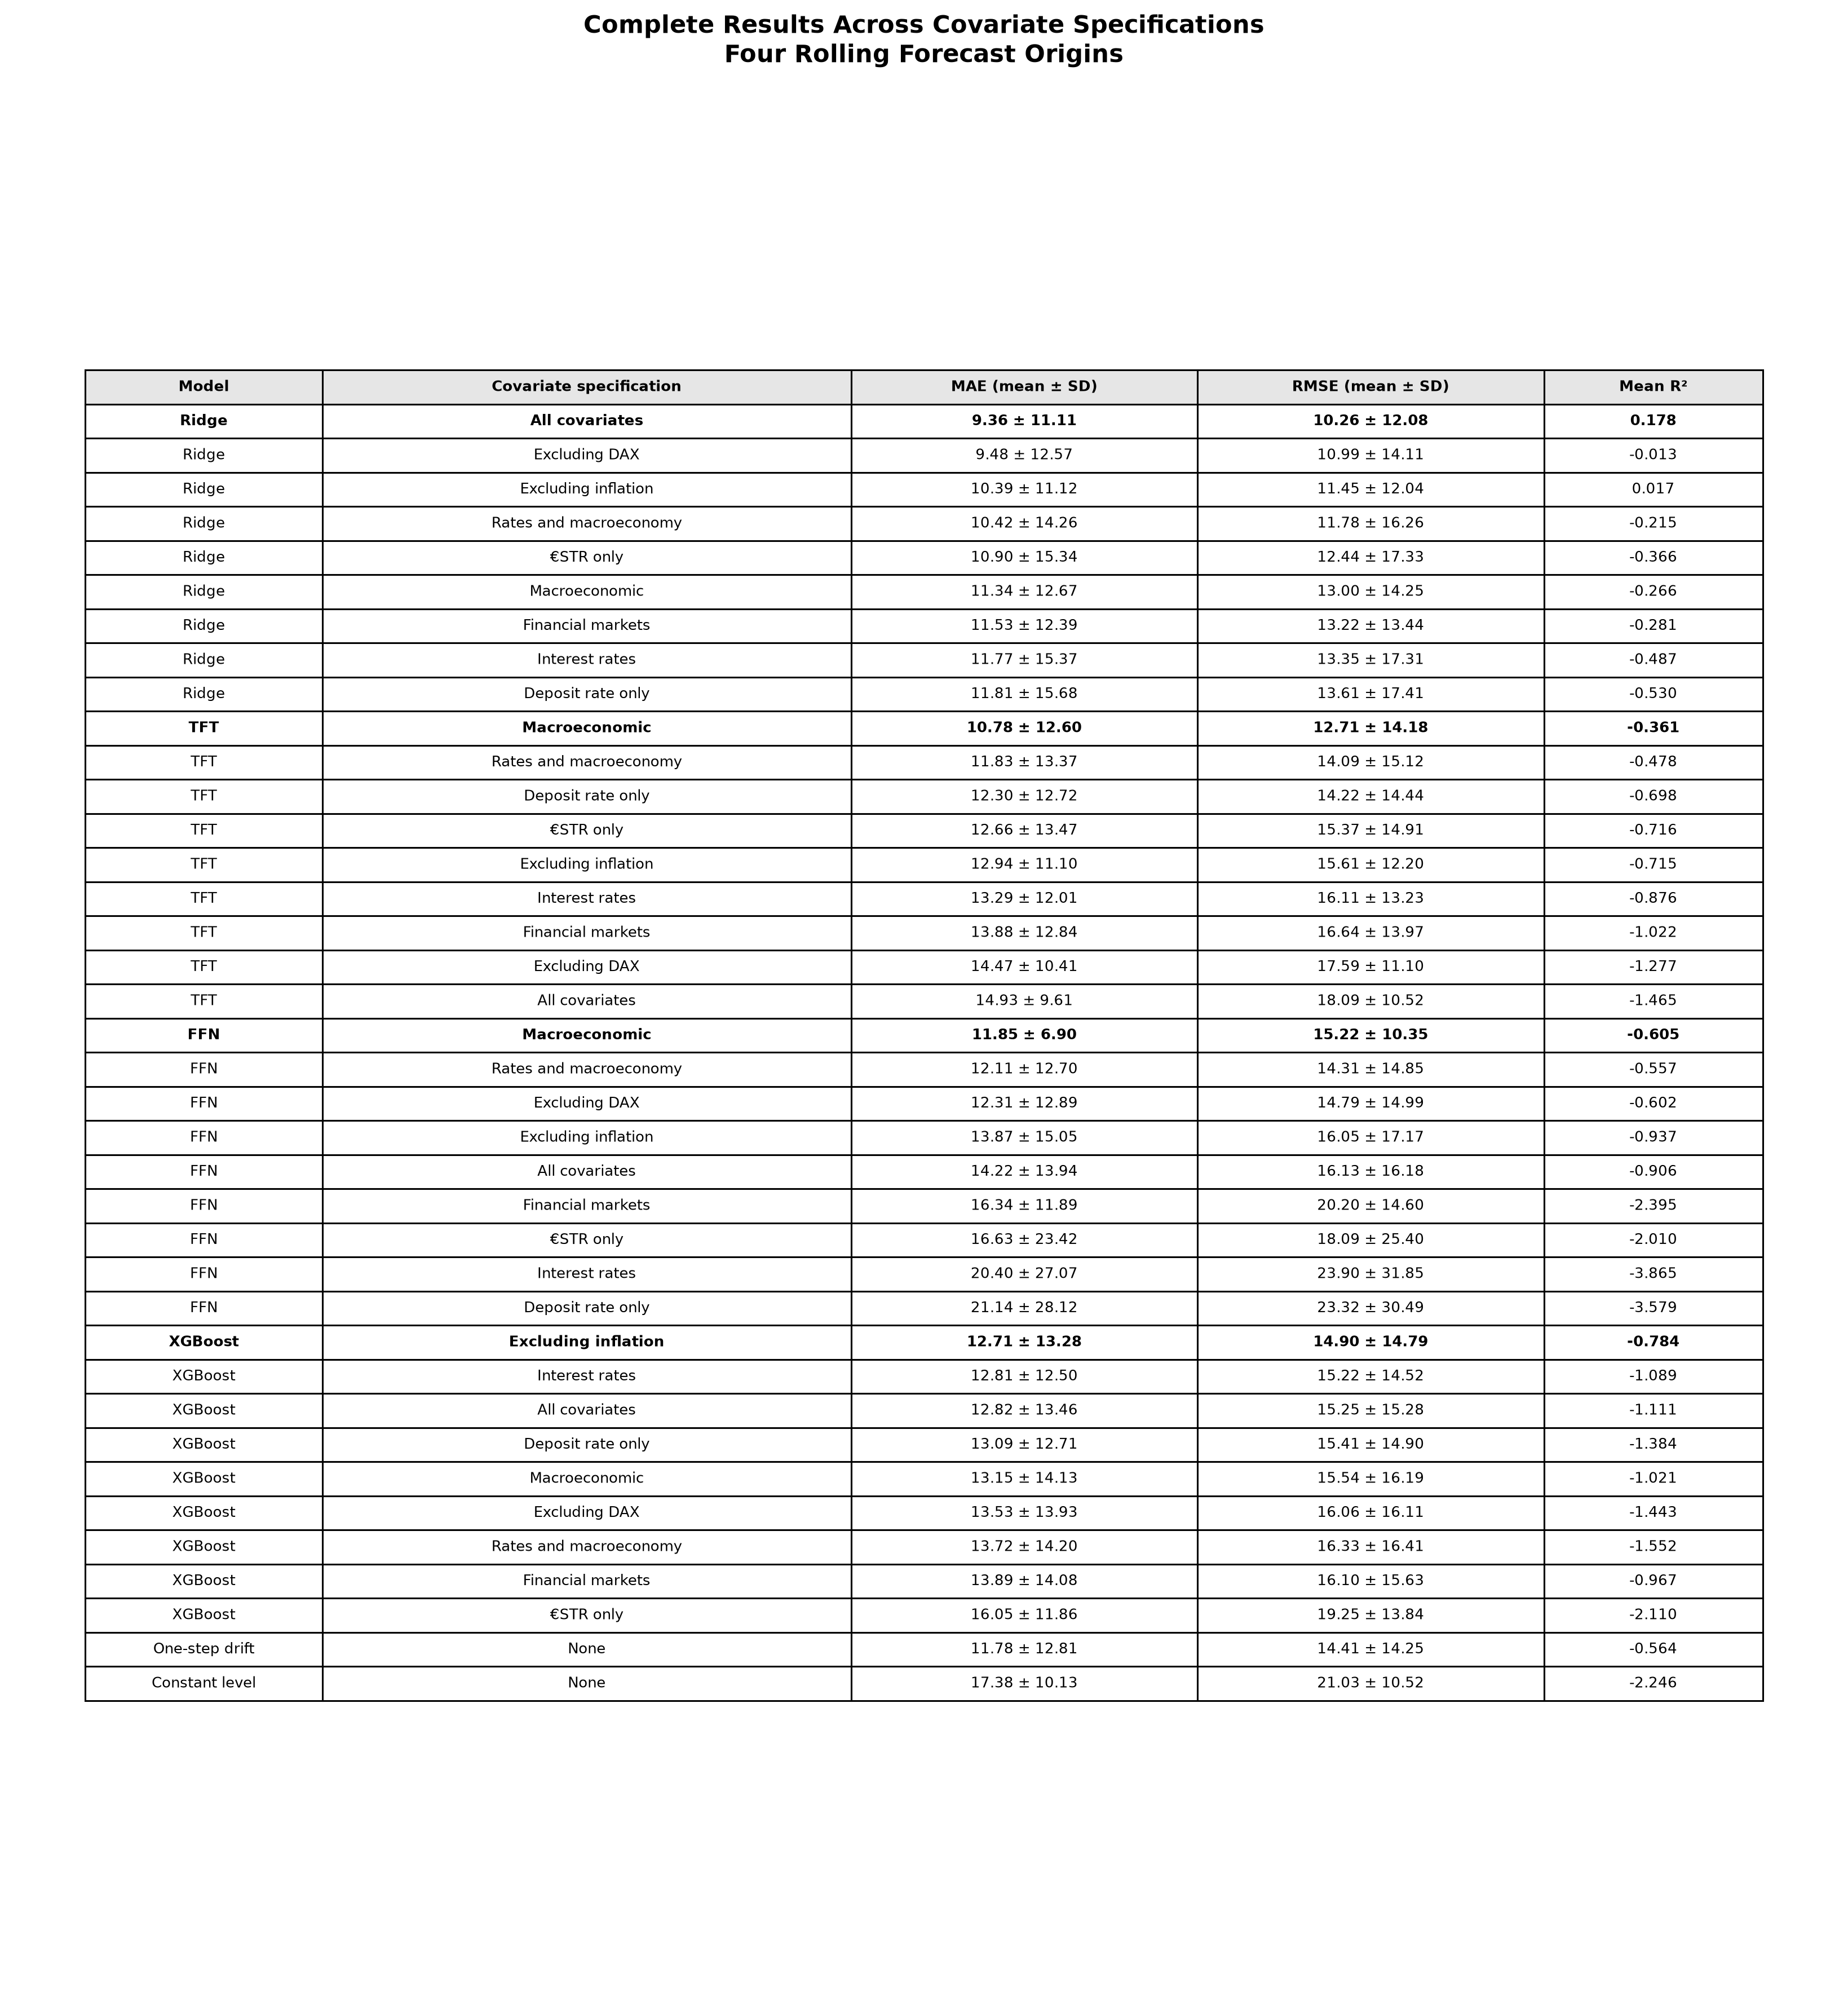
\includegraphics[width=\textwidth]{covariate_results_full.png}
    \caption{Complete forecasting results across the nine covariate
    specifications. MAE and RMSE are measured in EUR billions and reported
    as mean $\pm$ standard deviation across the four rolling forecast
    origins. Specifications are ordered by mean MAE within each model, and
    the best specification for each estimated model is shown in bold.}
    \label{fig:covariate_results_full}
\end{figure}

\originsgrid
  {forecast_ffn_nur_makro_2009-01-01.png}
  {forecast_ffn_nur_makro_2013-01-01.png}
  {forecast_ffn_nur_makro_2019-03-01.png}
  {forecast_ffn_nur_makro_2025-06-01.png}
  {FFN forecasts with the macroeconomic covariate set at all four rolling
   origins; panel construction as in Figure~\ref{fig:forecast_linreg}.}
  {fig:app_forecast_ffn}

\originsgrid
  {forecast_xgboost_nur_einlagezins_2009-01-01.png}
  {forecast_xgboost_nur_einlagezins_2013-01-01.png}
  {forecast_xgboost_nur_einlagezins_2019-03-01.png}
  {forecast_xgboost_nur_einlagezins_2025-06-01.png}
  {XGBoost forecasts with the deposit-rate-only specification at all four
   rolling origins; panel construction as in
   Figure~\ref{fig:forecast_linreg}. This is not the best-performing XGBoost
   specification (see Table~\ref{tab:overall_results}) but illustrates the
   extrapolation behaviour discussed in Section~\ref{sec:discussion} most
   clearly.}
  {fig:app_forecast_xgboost}

\begin{figure}[htbp]
    \centering
    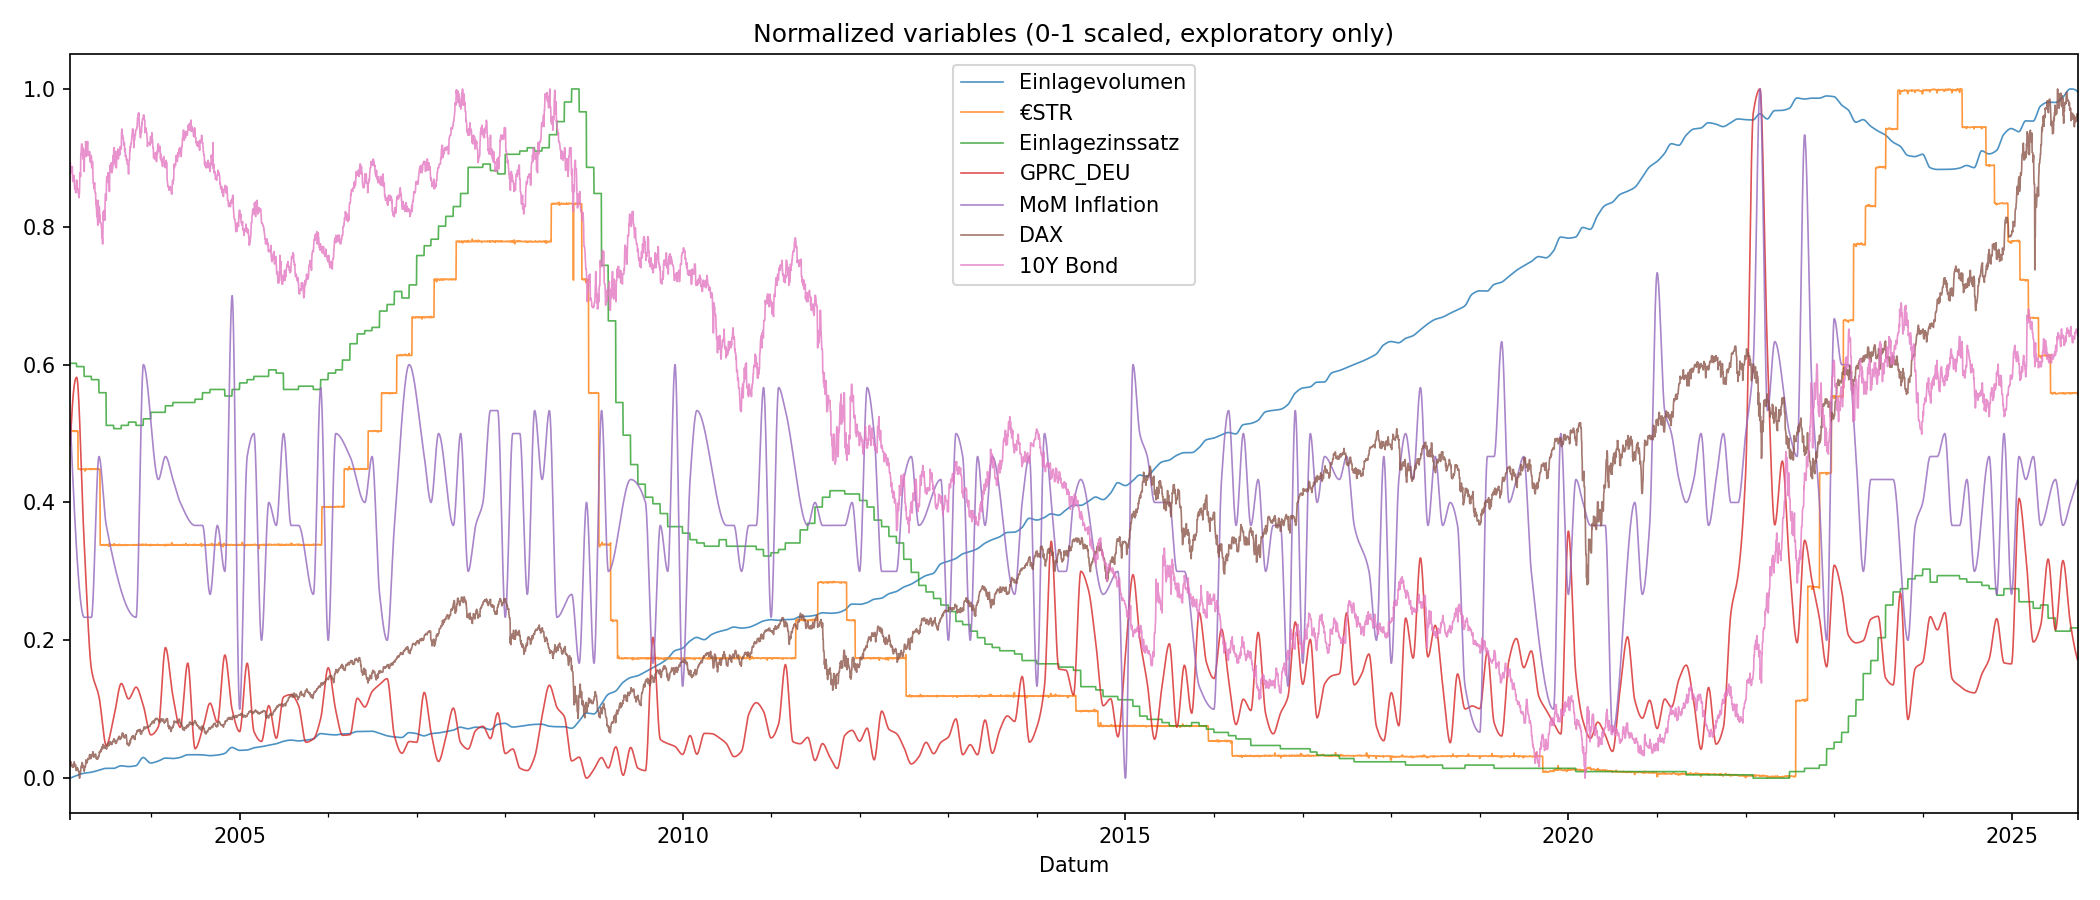
\includegraphics[width=0.9\textwidth]{overview_normalized.png}
    \caption{All variables after standardisation to zero mean and unit
    variance over the sample period January 2003 -- September 2025, shown on a
    common vertical scale so that co-movement between the deposit volume and
    the covariates is directly visible.}
    \label{fig:app_overview_normalized}
\end{figure}

\section{Appendix: Code}
\label{app:code}

The complete implementation, including the rolling-origin driver, the tuning
protocol of Table~\ref{tab:hyperparams}, and the scripts producing every
figure in this paper, is available in the accompanying repository. The excerpt
below shows the interface of the shared model-fitting routine.

\begin{lstlisting}[language=Python, caption={Shared model-fitting interface.}]
def fit_sequence_model(model_name, X_train, y_train, seed=SEED,
                       bootstrap=False, do_tune=False,
                       tuned_estimator=None):
    """Fit one ensemble member of a sequence model.

    model_name      : "linreg" | "ffn" | "xgboost"
    bootstrap       : resample training sequences (ensemble members S > 1)
    do_tune         : run the shared grid search (<= TUNING_BUDGET configs)
    tuned_estimator : reuse a cached configuration for the same origin
    """
    ...
\end{lstlisting}

\end{document}
